\documentclass[11pt,letterpaper]{report}
\usepackage[margin=0.75in]{geometry}
\usepackage[latin1]{inputenc}
\usepackage{amsmath}
\usepackage{amsfonts}
\usepackage{amssymb}
\usepackage{graphicx}
\usepackage{listings}	%needed for ls output
\usepackage{color}
\graphicspath{{./images/}{IR}}
\usepackage{fancyhdr}
\pagestyle{fancy}
\fancyhead{}
\lhead{CS333}
\chead{Project 5 Report}
\rhead{Andy Keene}
\author{Andy Keene}
\title{Project Five Report\\Introduction to Operating Systems\\ Spring 2017}
\date{}
\begin{document}
	\maketitle
	

	\section*{Description}
	For this assignment I learned about the file system abstraction in xv6; its underlying meta information; transactional operations in a log based file system; 
	and implemented a new simple file protection feature. This feature is conditionally compilable in its entirety and thus can be turned on or off. 
			
	\section*{Deliverables}
	The following features were added to xv6:

	\begin{itemize}
	
	
	\item Each file now contains the associated meta information for its owner ({\tt uid}), group ({\tt gid}), and permissions ({\tt mode}); the mode represents what read, write, and execute permissions the owner, group members, and others have along with a {\tt setuid} bit which indicates whether the process executing the file must inherit the files UID.  
	
	Thus, the {\tt inode}, {\tt dinode}, 
	and {\tt stat} structures were modified to contain this information while the kernel side functions {\tt ilock()}, {\tt iupdate()}, {\tt stati()} and {\tt create()} were modified to copy, return, and set
	this information as appropriate.
	
	\item The program {\tt mkfs} was modified to set all files owner, group, and mode to the default values upon creation of the xv6 file system. The default values are 0 for the owner and group
	and 0755 for the mode.
	\item New system calls to support file ownership and permissions:
	 	\begin{itemize}
			\item chmod sets the given {\tt mode}, or permission, bits for the target specified by {\tt pathname}.
				\begin{verbatim}
					int
					chmod(char *pathname, int mode);
				\end{verbatim}
				
			\item chown sets the UID for the file target specified by {\tt pathname} to the given {\tt owner}.
				\begin{verbatim}
					int
					chown(char *pathname, int owner);
				\end{verbatim}
			
			\item chgrp sets the GID for the file target specified by {\tt pathname} to the given {\tt group}.
				\begin{verbatim}
					int
					chgrp(char *pathname, int group);
				\end{verbatim}
					
		 \end{itemize}
	
	\item  Existing system calls were modified to both support and enforce file ownership and permissions. 
		The {\tt exec()} system call will first no longer read the file unless the calling process has execute permission for the file. Secondly, when the new image is omitted if the files setuid 
		mode bit is set, the executing process will inherit the files UID.  
			
	
	\item New user commands were added to give the user the ability to update a files UID, GID, and mode:
	
		\begin{itemize}
			\item {\tt chmod} sets the given mode, or permission, bits for file mode; where the file is specified by the {\tt target} pathname.
		
					Usage: {\tt chmod MODE TARGET}
					
			\item {\tt chown} sets the given owner as the file UID for the specified target; where target is a file path.
			
				Usage: {\tt chmod OWNER TARGET}
			\item {\tt chgrp} sets the given group as the file GID for the specified target; where target is a file path.
			
				Usage: {\tt chmod GROUP TARGET}
		\end{itemize}
	
%	\item The existing user command {\tt ls} was modified to now display, in total, the files mode, name, UID, GID, inode number, and size. The new output displays as:



	\item The existing user command {\tt ls} was modified to now display, in total the:
	
\subitem \texttt{mode}. The first column will display the mode bits for the file/directory/device. The first character indicates if the item is a regular file ('-'), directory ('d'), or device file ('c'). If the file is setuid, then the 'x' in the user permissions will be displayed as 'S'.
\subitem \texttt{name}. Name of the file or directory.
\subitem \texttt{uid}. User identifier (owner) of the file or directory.
\subitem \texttt{gid}. Group identifier (owning group) of the file or directory.
\subitem \texttt{inode}. Inode number of the file or directory.
\subitem \texttt{size}. Size in bytes of the file or directory. \\

The new output displays as:	
\noindent
\begin{lstlisting}
$ ls
mode            name    uid     gid     inode   size
drwxr-xr-x .              0     0       1       512
drwxr-xr-x ..             0     0       1       512
-rwxr-xr-x README         0     0       2       1973
-rwxr-xr-x cat            0     0       3       14884
-rwxr-xr-x echo           0     0       4       13849
-rwxr-xr-x forktest       0     0       5       9361
-rwxr-xr-x grep           0     0       6       16812
-rwxr-xr-x init           0     0       7       14750
-rwxr-xr-x kill           0     0       8       13981
-rwxr-xr-x ln             0     0       9       13879
-rwxr-xr-x ls             0     0       10      19010
-rwxr-xr-x mkdir          0     0       11      14010
-rwxr-xr-x rm             0     0       12      13991
-rwxr-xr-x sh             0     0       13      26855
-rwxr-xr-x stressfs       0     0       14      14969
-rwxr-xr-x usertests      0     0       15      69424
-rwxr-xr-x wc             0     0       16      15470
-rwxr-xr-x zombie         0     0       17      13615
-rwxr-xr-x halt           0     0       18      13441
-rwxr-xr-x MMchown        0     0       19      14464
-rwxr-xr-x MMchgrp        0     0       20      14464
-rwxr-xr-x MMchmod        0     0       21      14780
crwxr-xr-x console        0     0       22      0
$ ls halt
mode            name    uid     gid     inode   size
-rwxr-xr-x halt           0     0       18      13441
$
\end{lstlisting}

	
	
	\item Conditional compilation. Project 5 uses the {\tt CS333\_P5} flag, which may be turned on or turned off to enable the features outlined in this report.
		
	\end{itemize}
	
\newpage	
	\section*{Implementation}
	
	\subsection*{UID, GID, and Mode File Meta-information}
	To support the UID, GID, and Mode meta-information for files the {\tt inode}, {\tt dinode}, and {\tt stat} structures were updated with new fields. A new union definition, {\tt mode\_t},
	 to define the mode to be accessible as either bits or an int was added in fs.h (lines 32-49) as:
\begin{lstlisting}[language=C]
union mode_t {
  struct {
    uint o_x : 1;
    uint o_w : 1;
    uint o_r : 1;  // other
    uint g_x : 1;
    uint g_w : 1;
    uint g_r : 1;  // group
    uint u_x : 1;
    uint u_w : 1;
    uint u_r : 1;  // user
    uint setuid : 1;
    uint     : 22  // pad
  } flags;
  uint asInt;
};
\end{lstlisting}
	 The mode defines what read, write, and execute abilities that the owner, group, and others have for this file while the {\tt setuid} bit indicates whether the executing process must inherit
	 the files UID. 
	 The definitions for {\tt inode} and {\tt dinode} share this definition, while due to namespace issues, an identical copy to the definition above but named as {\tt stat\_mode\_t} was added
	 to stat.h (lines 5-22). Additionally, the fields {\tt ushort uid}, {\tt ushort gid}, and {\tt union mode\_t mode} were added to the {\tt dinode} and {\tt inode} structure definitions 
	 (fs.h lines 57-61, file.h lines 23-27). Due to the delicate balance a {\tt dinode}s size plays in the construction of the file system the number of {\tt dinodes}, NDIRECT, was modified to be
	 10 (fs.h lines 23-25) to accommodate the additional space each individual {\tt dinode} now occupies. For example, the new {\tt dinode} structure in total is now defined as (with conditional
	 compilation tags removed):

\begin{lstlisting}	 
struct dinode {
    short type;           // File type
    short major;          // Major device number (T_DEV only)
    short minor;          // Minor device number (T_DEV only)
    short nlink;          // Number of links to inode in file system
    ushort uid;           // owner ID
    ushort gid;           // group ID
    union mode_t mode;    // protection/mode bits
    uint size;            // Size of file (bytes)
    uint addrs[NDIRECT+1];   // Data block addresses
  };
 \end{lstlisting}
 	
	Similarly, the the fields {\tt ushort uid}, {\tt ushort gid}, and {\tt union stat\_mode\_t mode} were added to the {\tt stat} structure (stat.h lines 30-34).
	
	To support modifications to kernel side functions which must now set or update these fields in the respective structures, default values for the ownership (UID), groups (GID), and mode
	of a file were added to param.h (lines 14-18). These values for {\tt DEFAULT\_UID}, {\tt DEFAULT\_GID}, {\tt DEFAULT\_MODE}  were defined as 0, 0, and 0755 respectively. The default
	mode, 0755, defines permissions to be: the user can read, write and execute; the group and others can only read and execute; and the setuid bit is \emph{not} set. The inital
	process now has its UID and GID set using {\tt DEFAULT\_UID} and {\tt DEFAULT\_GID} values rather than the old definitions which implied the use was exclusively for the
	initial process (proc.c 496-497).
	
	The following kernel side functions were modified to support the copying of this information between file abstraction structures, and initializing these fields on creation:
	\begin{itemize}
		
		\item {\tt ilock}. {\tt ilock()} is responsible for setting a lock on the inode reference and updating the inodes information with its corresponding on-disk dinode. As such, 
			{\tt ilock()} now copies the {\tt uid}, {\tt gid}, and {\tt mode} fields from the dinode \emph{to} the inode (fs.c lines 294-299).
		\item {\tt iupdate}. {\tt iupdate()} is responsible for refreshing the corresponding dinode with changes to the given inode. As such, {\tt ilock()} now copies 
			the {\tt uid}, {\tt gid}, and {\tt mode} fields from the inode \emph{to} the dinode (fs.c lines 211-216).
		\item {\tt stati}. {\tt stati()} is invoked deep within the {\tt fstat} system call and is responsible for copying inode information to the stat structure. As such, {\tt stati()} now copies 
			the {\tt uid}, {\tt gid}, and {\tt mode} fields from the inode \emph{to} the stat structure (fs.c lines 211-216).
		\item {\tt create}. {\tt create()} is invoked by system calls responsible for creating a file or directory - the inode structure created now has its {\tt uid} field set to be that of the calling
			process, the {\tt gid} field to be that of the calling process, and the {\tt mode} field to be the default of 0755 (sysfile.c lines 265-273). It should be noted that the rationale for
			setting the UID and GID to the calling process is that the calling process is the files owner - and thus should be linked by default in this manor. This establishes basic permission
			restrictions - i.e. only the \emph{user} or rather owner, may edit the file by default.
	
	

	\end{itemize} 
	
	\subsection*{mkfs}
	The program {\tt mkfs} is responsible for building the xv6 file system on boot if it is not already built. When a file is created the {\tt ialloc()} function call within {\tt mkfs} is invoked and sets properties
	such as {\tt type}, {\tt nlink} (number of links), and {\tt size} for the {\tt dinode} before it is written to disk; here default values for the {\tt uid}, {\tt gid}, and {\tt mode} are now set for the
	 {\tt dinode} (mkfs.c lines 233-338) before writing to disk. Additionally, a project 5 conditional compilation flag ({\tt CS333\_P5}) was added to the mkfs make target (Makefile line 133) since this does not use 
	 the CFLAGS variable responsible for flagging conditional compilation for the rest of the files. The original target can still be set by swapping line 133 with the original target which is commented out 
	 on line 134 of the Makefile. 
	
	
	\subsection*{New System Calls}
	Using the process outlined in project one, the following system calls were implemented by adding: a user-side header in {\tt user.h}; 
	creating a system call number in {\tt syscall.h}; updating the system call jump table, the system call name table, and adding a kernel side
	header in {\tt syscall.c}; 
	a user-side stub in {\tt usys.S}; and implementation in {\tt sysfile.c} since the system call is responsible for handling file information. 
	
	Each of the following system calls is responsible for updating a files meta data on disk. Thus, all follow a transactional procedure. The transaction procedure begins by
	 calling {\tt begin\_op()} to instantiate a transaction with the
	file system. The procedure then attempts to aquire the inode for the given \emph{pathname} via a call to the kernel side {\tt namei()} where if the inode is not found, the transaction is ended with a call to {\tt end\_op()} and -1
	is returned. Upon successfully retrieving the inode for the \emph{pathname} it is locked for the purpose of atomicity using {\tt ilock()}. The appropriate inode meta information is then updated before  
	{\tt iupdate()} is called to sync the changes to the inode with the disk. Lastly, the transaction is ended with a call to {\tt end\_op()} and 0 is returned to signal a successful update of the files meta information.



        Each new system call's description and it's corresponding file changes are as follows:

		\begin{itemize}

			\item The {\tt chmod()} system call sets the mode of the given file \emph{pathname}, to the given \emph{mode}. The given \emph{mode}
				is retrieved from the stack as an int using {\tt argint()} while the targets \emph{pathname} is retrieved using  {\tt argptr()}; if {\tt chmod()} fails to retrieve
				either of the arguments, or if the successfully retrieved \emph{mode} is greater than the octal representation 0755 or less than 0, then -1 is returned to signal an error.
				Upon successfully retrieving the arguments from the stack and validating the {\tt mode}s range, {\tt chmod()} follows the transactional procedure outlined above where 
				the file meta information updated is the inodes {\tt mode}.
							 
				 The files modified to support this system call are as follows:				
					\begin{itemize}
										
					\item user.h (line 42)
					\item usys.S (line 41)
					\item syscall.h (line 34)
					\item syscall.c (lines 111, 148, 188)
					\item sysfile.c (lines 456-486)
					
					\end{itemize}
			
				The function prototype is:
				\begin{verbatim}
					int
					chmod(char *pathname, int mode);
				\end{verbatim}

			\item The {\tt chown()} system call sets the UID of the given file \emph{pathname}, to the given \emph{owner}. The given \emph{owner}
				is retrieved from the stack as an int using {\tt argint()} while the targets \emph{pathname} is retrieved using  {\tt argptr()}; if {\tt chown()} fails to retrieve
				either of the arguments, or if the successfully retrieved \emph{owner} is greater than the maximum UID (32767) or less than 0, then -1 is returned to signal an error.
				Upon successfully retrieving the arguments from the stack and validating the {\tt owner}s range, {\tt chown()} follows the transactional procedure outlined above where 
				the file meta information updated is the inodes {\tt uid}.
							 
				 The files modified to support this system call are as follows:				
					\begin{itemize}
										
					\item user.h (line 43)
					\item usys.S (line 42)
					\item syscall.h (line 35)
					\item syscall.c (lines 112, 149, 189)
					\item sysfile.c (lines 488-519)
					
					\end{itemize}
			
				The function prototype is:
				\begin{verbatim}
					int
					chown(char *pathname, int owner);
				\end{verbatim}
				
				
			\item The {\tt grp()} system call sets the UID of the given file \emph{pathname}, to the given \emph{group}. The given \emph{group}
				is retrieved from the stack as an int using {\tt argint()} while the targets \emph{pathname} is retrieved using  {\tt argptr()}; if {\tt chgrp()} fails to retrieve
				either of the arguments, or if the successfully retrieved \emph{group} is greater than the maximum GID (32767) or less than 0, then -1 is returned to signal an error.
				Upon successfully retrieving the arguments from the stack and validating the {\tt group}s range, {\tt chgrp()} follows the transactional procedure outlined above where 
				the file meta information updated is the inodes {\tt gid}.
							 
				 The files modified to support this system call are as follows:				
					\begin{itemize}
										
					\item user.h (line 44)
					\item usys.S (line 43)
					\item syscall.h (line 36)
					\item syscall.c (lines 113, 150, 190)
					\item sysfile.c (lines 521-552)
					
					\end{itemize}
			
				The function prototype is:
				\begin{verbatim}
					int
					chgrp(char *pathname, int group);
				\end{verbatim}
				
									
		\end{itemize} 
	
	\subsection*{Modified system calls - exec()}
	The system call {\tt exec()} was modified to enforce the permissions set by the mode of a file when executing a file. To support this the headers for fs.h and file.h (in order) were included to give {\tt exec()} the ability to see and use
	the inode structures relevant fields (lines 12-13). {\tt exec()} now uses the permissions associated with the group the process belongs to (exec.c lines 46-59); that is in-order, if the calling process and the file have the same UID, 
	the modes \emph{user} permissions are used;
	if the calling process and the file have the same GID, the modes \emph{group} permissions are used; if the calling process and the file have neither the same UID nor GID then the modes \emph{other} permissions are used. 
	
	If the permission group to 
	which the calling process belongs \emph{does not} have executable permissions (i.e. the {\tt x} bit is not set) then the file is not read and {\tt exec()} jumps to the {\tt bad} routine which cleans up the opened resources and returns -1. However, 
	if the process has executable permissions, as outlined, then the {\tt setuid} of the file is checked (lines 63-64) where if this mode bit is set then the file UID is saved and later used to set the calling process UID immediately before execution of the file begins
	(lines 129-130). Note that {\tt setuid} is initialized as -1 since this is an illegal UID and thus indicates, if unchanged, that the process UID \emph{should not} be set before execution.
	
	\subsection*{New User Commands}
	All user commands wrapped the operating code in conditional compilation tags, so that if the project 5 flag is not set but the user programs are not removed from the Makefile, their execution will do nothing.
	
	\begin{itemize}
	
		\item The {\tt chmod} user command (chmod.c) first verifies it is given both a \emph{mode} and filepath \emph{target} argument, and that the \emph{mode} is exactly four digits (lines 12-20). If these conditions are not met a usage message is printed to standard
			out and the program exits. The string representing the \emph{mode} is then parsed using a routing similar to the user library function {\tt atoi()} (lines 25-33), where all octal characters are converted to an integer and if the character is not valid a usage
			message is printed to the screen and the program exits. Consequently, an integer representing the octal character string is created \emph{iff} all characters in the string are valid octal numbers (0-7). Note that although this does not necessarily ensure a correct mode
			the system call {\tt chmod()} validates the mode independently. The integer representing the octal given \emph{mode} and the \emph{target} are then passed to the {\tt chmod()} system call; where if this call 
			returns an error a message is printed to standard out (35-36). 
			{\tt chmod} was added to the Makefile user programs (line 163).
			
			Usage: {\tt chmod MODE TARGET}
			
		\item The {\tt chown} user command (chown.c) validates it is given both an \emph{owner} and filepath \emph{target} (lines 11-14). It then passes the given \emph{owner}, converted to an integer using the user side function {\tt atoi()}, and the \emph{target} 
			argument to the {\tt chown()} system call (lines 18-19). If the call fails, a message is printed to standard out before the program exits (lines 18-19).
			{\tt chown} was added to the Makefile user programs (line 164).
			
			Usage: {\tt chown OWNER TARGET}
			
		\item The {\tt chgrp} user command (chgrp.c) validates it is given both a \emph{group} and filepath \emph{target} target(lines 11-14). It then passes the given \emph{group}, converted to an integer using the user side function {\tt atoi()}, and the \emph{target} 
			argument to the {\tt chgrp()} system call (lines 18-19). If the call fails, a message is printed to standard out before the program exits (lines 19-21).
			{\tt chgrp} was added to the Makefile user programs (line 165).
			
			Usage: {\tt chgrp GROUP TARGET}
			

	\end{itemize}
	
	\subsection*{ls Modification}
	Due to the modifications in the stat.h and the {\tt stati()} system call described in the \emph{UID, GID, and Mode File Meta-information} section, the {\tt fstat()} system call returns a stat structure that contains the files
	{\tt uid}, {\tt gid}, and {\tt mode}. As such, the only modifications necessary to update the display information in {\tt ls} was the printing routine. The print\_mode.c routine that was provided is now included in ls.c (line 6); 
	 this routine is responsible for displaying the mode in the form of {\tt -rwx-r-xr-x} where: the first character indicates if the item is a regular file ('-'), directory ('d'), or device file ('c'); if the file is setuid, then the 'x' in the 
	 user permissions will be displayed as 'S'; and the right nine spots indicate the user, group and other permissions (i.e. {\tt -uuugggooo}). Line 49 is now responsible for printing a header to identify the respective columns, where
	 lines 55-56 and lines 80-81 now print the new information for files and directories. As discussed in the \emph{Deliverables} section, the information for each file and directory that is printed, in total includes the mode, name, 
	 uid, gid, inode number, and size. The new output displays as:
	 
	  \noindent
\begin{lstlisting}
$ ls
mode            name    uid     gid     inode   size
drwxr-xr-x .              0     0       1       512
drwxr-xr-x ..             0     0       1       512
-rwxr-xr-x README         0     0       2       1973
-rwxr-xr-x cat            0     0       3       14884
-rwxr-xr-x echo           0     0       4       13849
-rwxr-xr-x forktest       0     0       5       9361
-rwxr-xr-x grep           0     0       6       16812
-rwxr-xr-x init           0     0       7       14750
-rwxr-xr-x kill           0     0       8       13981
-rwxr-xr-x ln             0     0       9       13879
-rwxr-xr-x ls             0     0       10      19010
-rwxr-xr-x mkdir          0     0       11      14010
-rwxr-xr-x rm             0     0       12      13991
-rwxr-xr-x sh             0     0       13      26855
-rwxr-xr-x stressfs       0     0       14      14969
-rwxr-xr-x usertests      0     0       15      69424
-rwxr-xr-x wc             0     0       16      15470
-rwxr-xr-x zombie         0     0       17      13615
-rwxr-xr-x halt           0     0       18      13441
-rwxr-xr-x MMchown        0     0       19      14464
-rwxr-xr-x MMchgrp        0     0       20      14464
-rwxr-xr-x MMchmod        0     0       21      14780
crwxr-xr-x console        0     0       22      0
$ ls halt
mode            name    uid     gid     inode   size
-rwxr-xr-x halt           0     0       18      13441
\end{lstlisting}	


	\newpage
	
	
	
	\section*{Testing}
	
	\subsection*{System calls}
	All system calls - {\tt setuid()}, {\tt setgid()}, {\tt chmod()}, {\tt chgrp()}, {\tt chown()}, {\tt exec()} -  
	were tested using the provided automated test suite {\tt p5-test}. 
	The following subsections, one for each system call, will describe: what is to be tested; how the {\tt p5-test} harness runs the test; what the expected results are; 
	what the results are; and if the results demonstrate the correct behavior for the system call. The main loop (lines 344-355) prints a menu with options 0-7 invoking the corresponding test
	function by calling {\tt doTest()} which runs the given function name with the given argument; this is either the empty string or the name of the file {\tt setsetuid} which 
	will simply print the UID of its process. Unless noted otherwise, a secondary helper function {\tt check()} is used to run all system calls with arbitrary arguments and both prints an error 
	message and 
	aborts when the command
	invoked (i.e. {\tt exec()}) returns an error code. Thus anytime {\tt check()}, or a system call, is called in subsequent tests, we know the program will inform us and abort when an 
	error code is returned. Since some of the tests within {\tt p5-test} depend on default permissions for the file each test will only be run immediately after a make and boot of xv6.
	
	\subsection{setuid()}
	This test will demonstrate the correct behavior of the {\tt setuid()} system call. To do this, we will run {\tt p5-test} immediately after the make and boot of xv6 
	and press 1 to trigger the function {\tt doUidTest()} with a null argument (described previously in \emph{0.0 System Calls}). 

	{\tt doUidTest()} will first get and save the UID of its process. Next it will increment this value by 1 and set this as its UID through the {\tt setuid()} system call where if the return code 
	signals an error occurred the test quite will print a report and abort. Note that since no UIDs will have been changed previous to the test running and all processes inherit their UID from their parent with the exception
	of {\tt initproc()} whose UID is set to the default value 0, we know the increment by 1 will be a valid UID. {\tt doUidTest()} will then verify this UID was set correctly by calling {\tt getuid()} and comparing the returned value against
	what it set the UID to be; here if a match is not found {\tt p5-test} will error and abort. Lastly, for the list of invalid UIDs -  32767+5, -41, \~0 - the test will validate an error code is returned
	by {\tt setuid()} if any are used as an argument - any successful return code will cause {\tt p5-test} to error and abort. Since {\tt doUidTest()} errors and aborts at any incorrect behavior and demonstrates both 
	valid and invalid UIDs are set or handled correctly, we expect if {\tt setuid()} is correct that {\tt doUidTest()} will complete and prints that the test was successful.
	
	
\begin{figure}[h!]
\centering
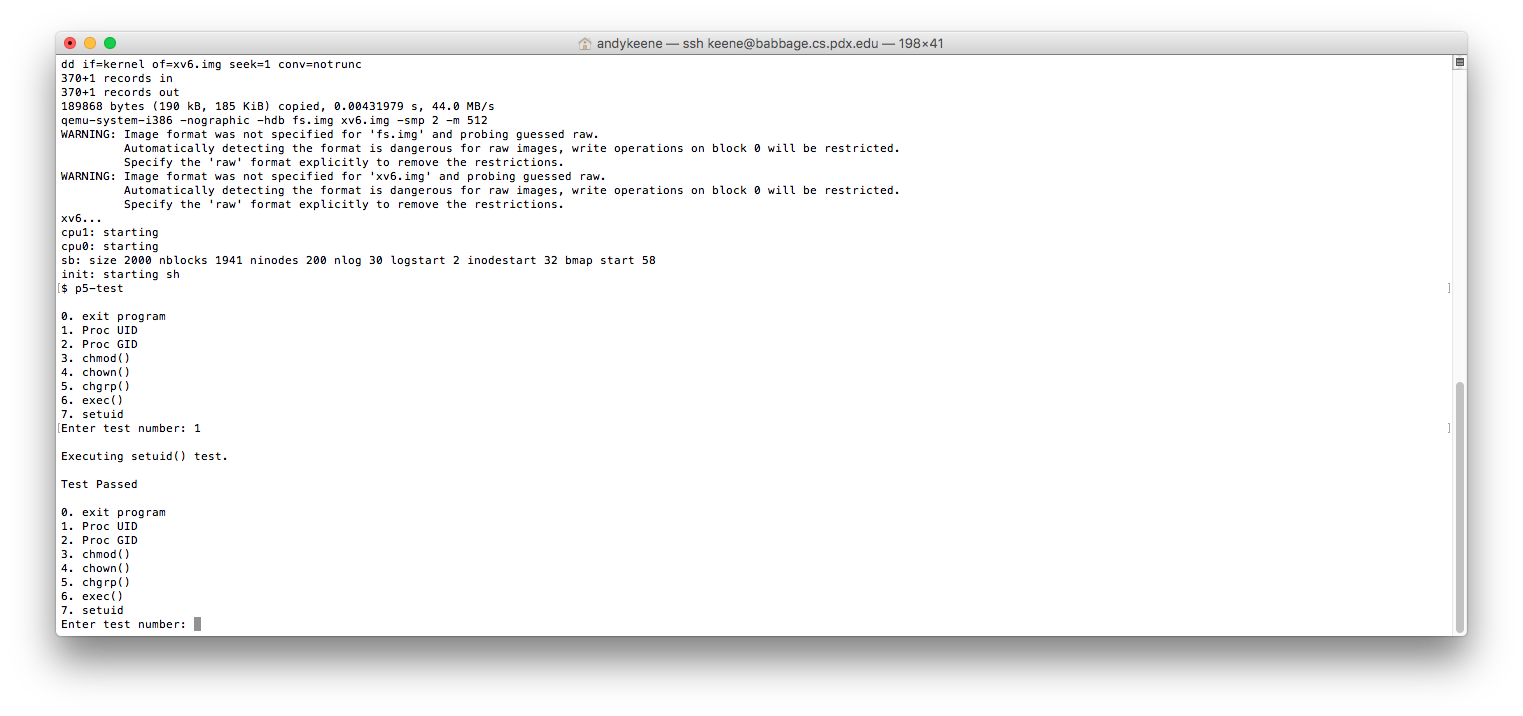
\includegraphics[width=0.8\linewidth]{douidtest.png}
\caption{p5-test option 1: doUidTest()}
\label{fig:datetest}
\end{figure}
	
	Here we see that upon booting xv6 that {\tt p5-test} was immediately run with option 1 invoking the {\tt doUidTest()}. Since the completion of the test, by virtue of the code outlined above, demonstrates
	the correct behavior of {\tt setuid()} we can conclude that this sub-test \textbf{PASSES}.
		
	\subsection{setgid()}
	This test will demonstrate the correct behavior of the {\tt setgid()} system call. To do this, we will run {\tt p5-test} immediately after the make and boot of xv6 
	and press 2 to trigger the function {\tt doGidTest()} with a null argument (described previously in \emph{0.0 System Calls}). 

	{\tt doGidTest()} will first get and save the GID of its process. Next it will increment this value by 1 and set this as its GID through the {\tt setgid()} system call where if the return code 
	signals an error occurred the test quite will print a report and abort. Note that since no GIDs will have been changed previous to the test running and all processes inherit their GID from their parent with the exception
	of {\tt initproc()} whose GID is set to the default value 0, we know the increment by 1 will yield a valid GID.
	{\tt doGidTest()} will then verify this GID was set correctly by calling {\tt getgid()} and comparing the returned value against
	what it set the GID to be; here if a match is not found, another {\tt p5-test} will error and abort. Lastly, for the list of invalid GIDs -  32767+5, -41, \~0 - the test will validate an error code is returned
	by {\tt setgid()} if any are used as an argument - any successful return code will cause {\tt p5-test} to error and abort. Since {\tt doGidTest()} errors and aborts at any incorrect behavior and demonstrates both 
	valid and invalid UIDs are set or handled correctly, we expect if {\tt setgid()} is correct that {\tt doGidTest()} will complete and prints that the test was successful.

\begin{figure}[h!]
\centering
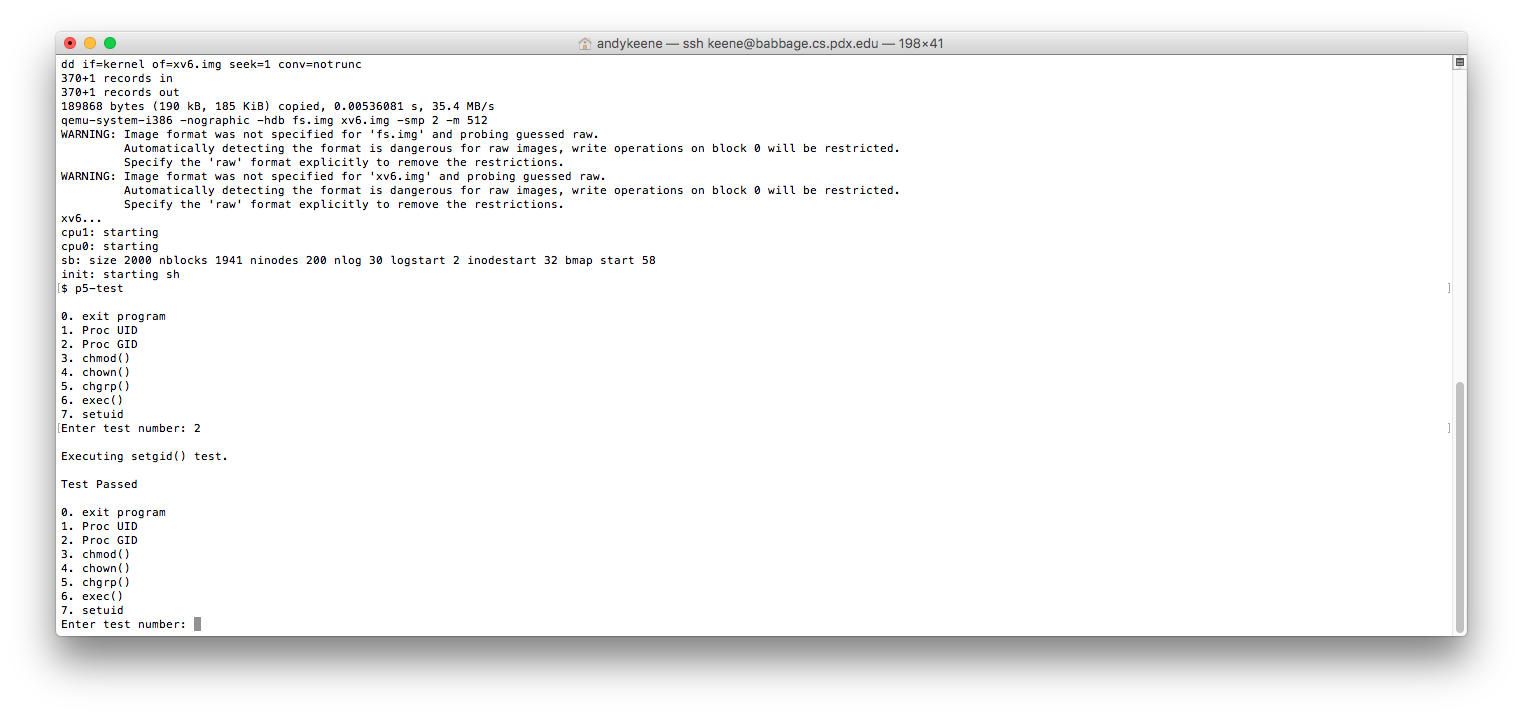
\includegraphics[width=0.8\linewidth]{dogidtest.png}
\caption{p5-test option 2: doGidTest()}
\label{fig:datetest}
\end{figure}

	Here we see that upon booting xv6 that {\tt p5-test} was immediately run with option 2 invoking the {\tt doGidTest()}. Since the completion of the test, by virtue of the code outlined above, demonstrates
	the correct behavior of {\tt setgid()} we can conclude that this sub-test \textbf{PASSES}.

	
	\subsection{chmod()}
	This test will demonstrate the correct behavior of {\tt chmod()}. To do this, we will run {\tt p5-test} immediately after the boot of xv6 
	and press 3 to trigger the function {\tt doChmodTest()} with an argument of 
	{\tt testsetuid} (described previously in \emph{0.0 System Calls}). 
	
	{\tt doChmodTest()} (lines 164-197)  gets file meta information for testsetuid by calling {\tt (stat()} and saves its current mode. Next, for each of the permissions 1544, 1454, 1445, 1666,
	{\tt doChmodTest()} sets permissions for the file testsetuid and refreshes the file information by calling {\tt stat()} again on the stat structure it holds. If the mode from 
	the file meta information after the refresh matches the original permissions it saved, or if the refreshed mode does not match the mode given to the last invocation of {\tt chmod()} 
	(addition to lines 195-199) then the function will print an error message and exit. After all the permissions listed have been tested {\tt doChmodTest()} will print that the test passed and
	return the the main menu. 
	
	Since the correct behavior of {\tt chmod()} is to set a \emph{valid} mode for the given file if it exists,
	and we know that the file exists, that each mode is valid, and that the file will have the default permissions of 0755 which isn't listed in the tested permissions - 
	we expect for the test to run without any error messages and to print that the test passed before
	it exits after completion.
	
\begin{figure}[h!]
\centering
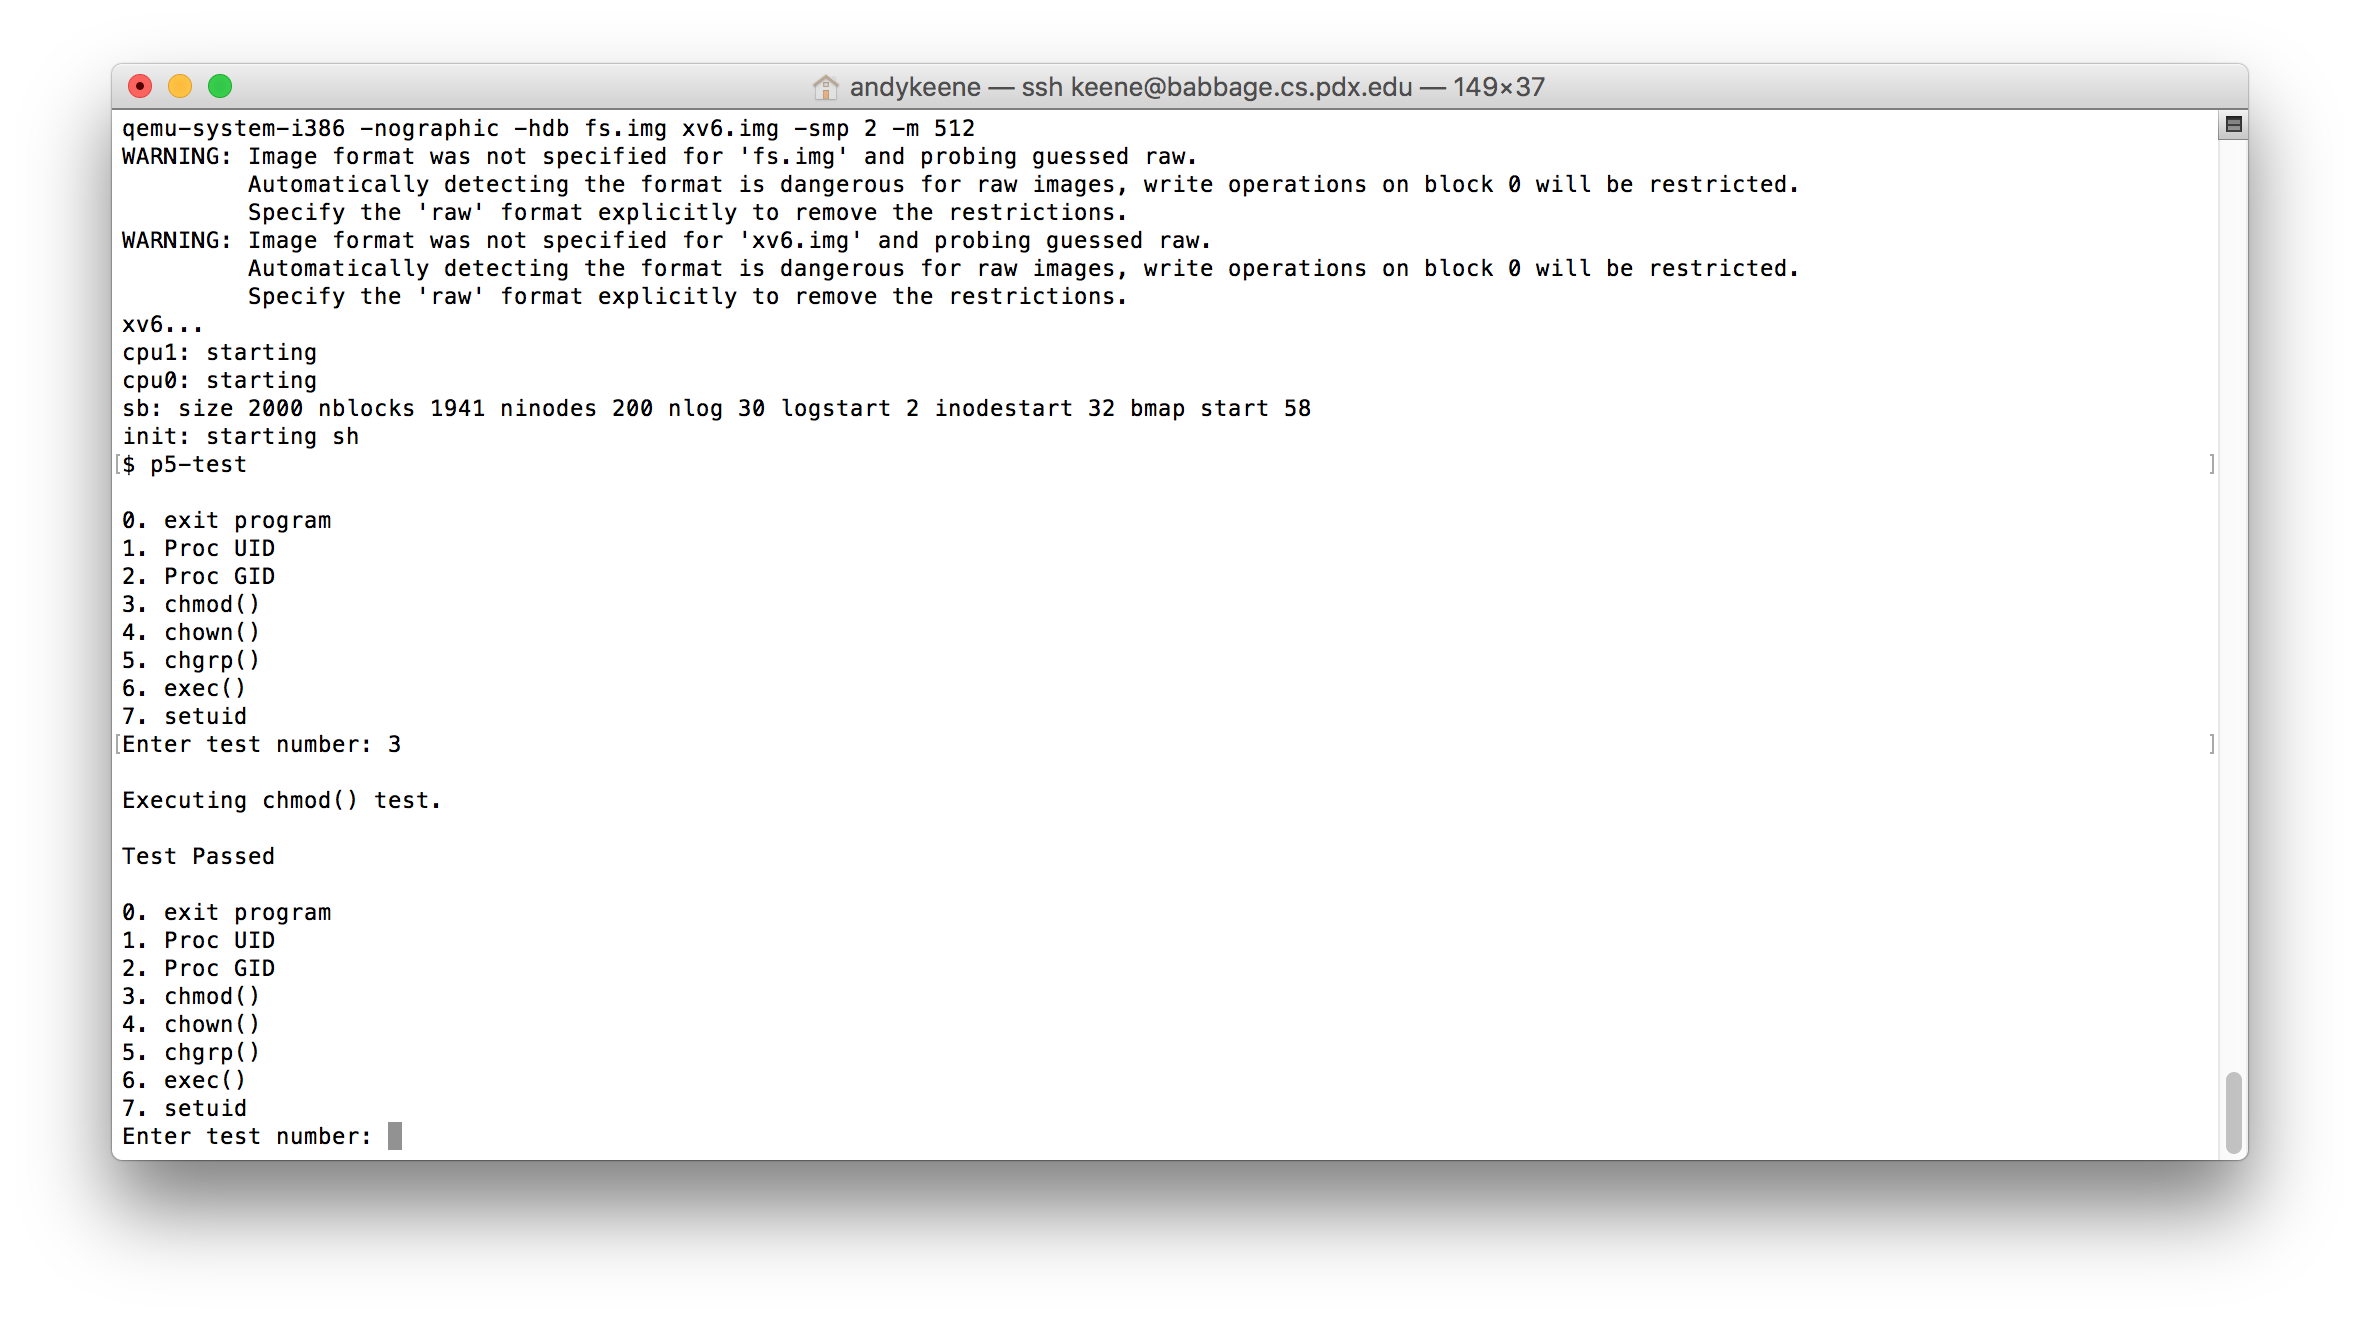
\includegraphics[width=0.8\linewidth]{dochmodtest.png}
\caption{p5-test option 3: doChmodTest()}
\label{fig:datetest}
\end{figure}

\pagebreak
Here we see that upon boot of xv6 that the program {\tt p5-test} was immediately run, and that by pressing 3 we invoked the specific test for {\tt doChmodTest()}. Next we see that the test ran without
errors and that control was returned to the main menu as expected. Thus, since our expectations for this sub-test were met, this sub-test \textbf{PASSES}.


	\subsection{chown()}
	This test will demonstrate the correct behavior of the {\tt chown()} system call. To do this, we will run {\tt p5-test} immediately after the make and boot of xv6 
	and press 4 to trigger the function {\tt doChownTest()} with an argument of {\tt testsetuid} (described previously in \emph{0.0 System Calls}). 
	
	 {\tt doChownTest()} will notify us that is is executing then get the meta information for the file testsetuid by calling {\tt stat}. Next it will save the original UID, uid1, of
	 testsetuid before calling {\tt chown()} with an owner argument of uid1+1. Since during the file system creation all files are given a UID of $DEFAULT\_UID$ 
	 (demonstrated in test mkfs) which we 
	 know by virtue of code to be defined as 0 we can conclude that uid1+1 will in fact be within the valid bounds for a UID and consequently, the system call should succeed.
	 {\tt doChownTest()} then checks the return code of {\tt chown()} where an error message will be printed if the return code corresponds to an error. The file meta information
	 for testtestuid will then be refreshed with another call to stat. Using the stat structure, {\tt doChownTest()} will then ensure that the refreshed UID of the file matches the original
	 UID +1, or uid1+1 (this addition to the test occurs on line 226). Before returning control to the main loop {\tt doChownTest()} will reset the original file UID and print a message of success.
	 
	 We expect that after making and booting xv6 that when {\tt p5-test} is run and option 4 is selected that we will see only a message that {\tt doChownTest()} is running and 
	 a message that the test passed - by virtue of the code described for this test, will will know {\tt chown()} correctly updated the UID.
	 
\begin{figure}[h!]
\centering
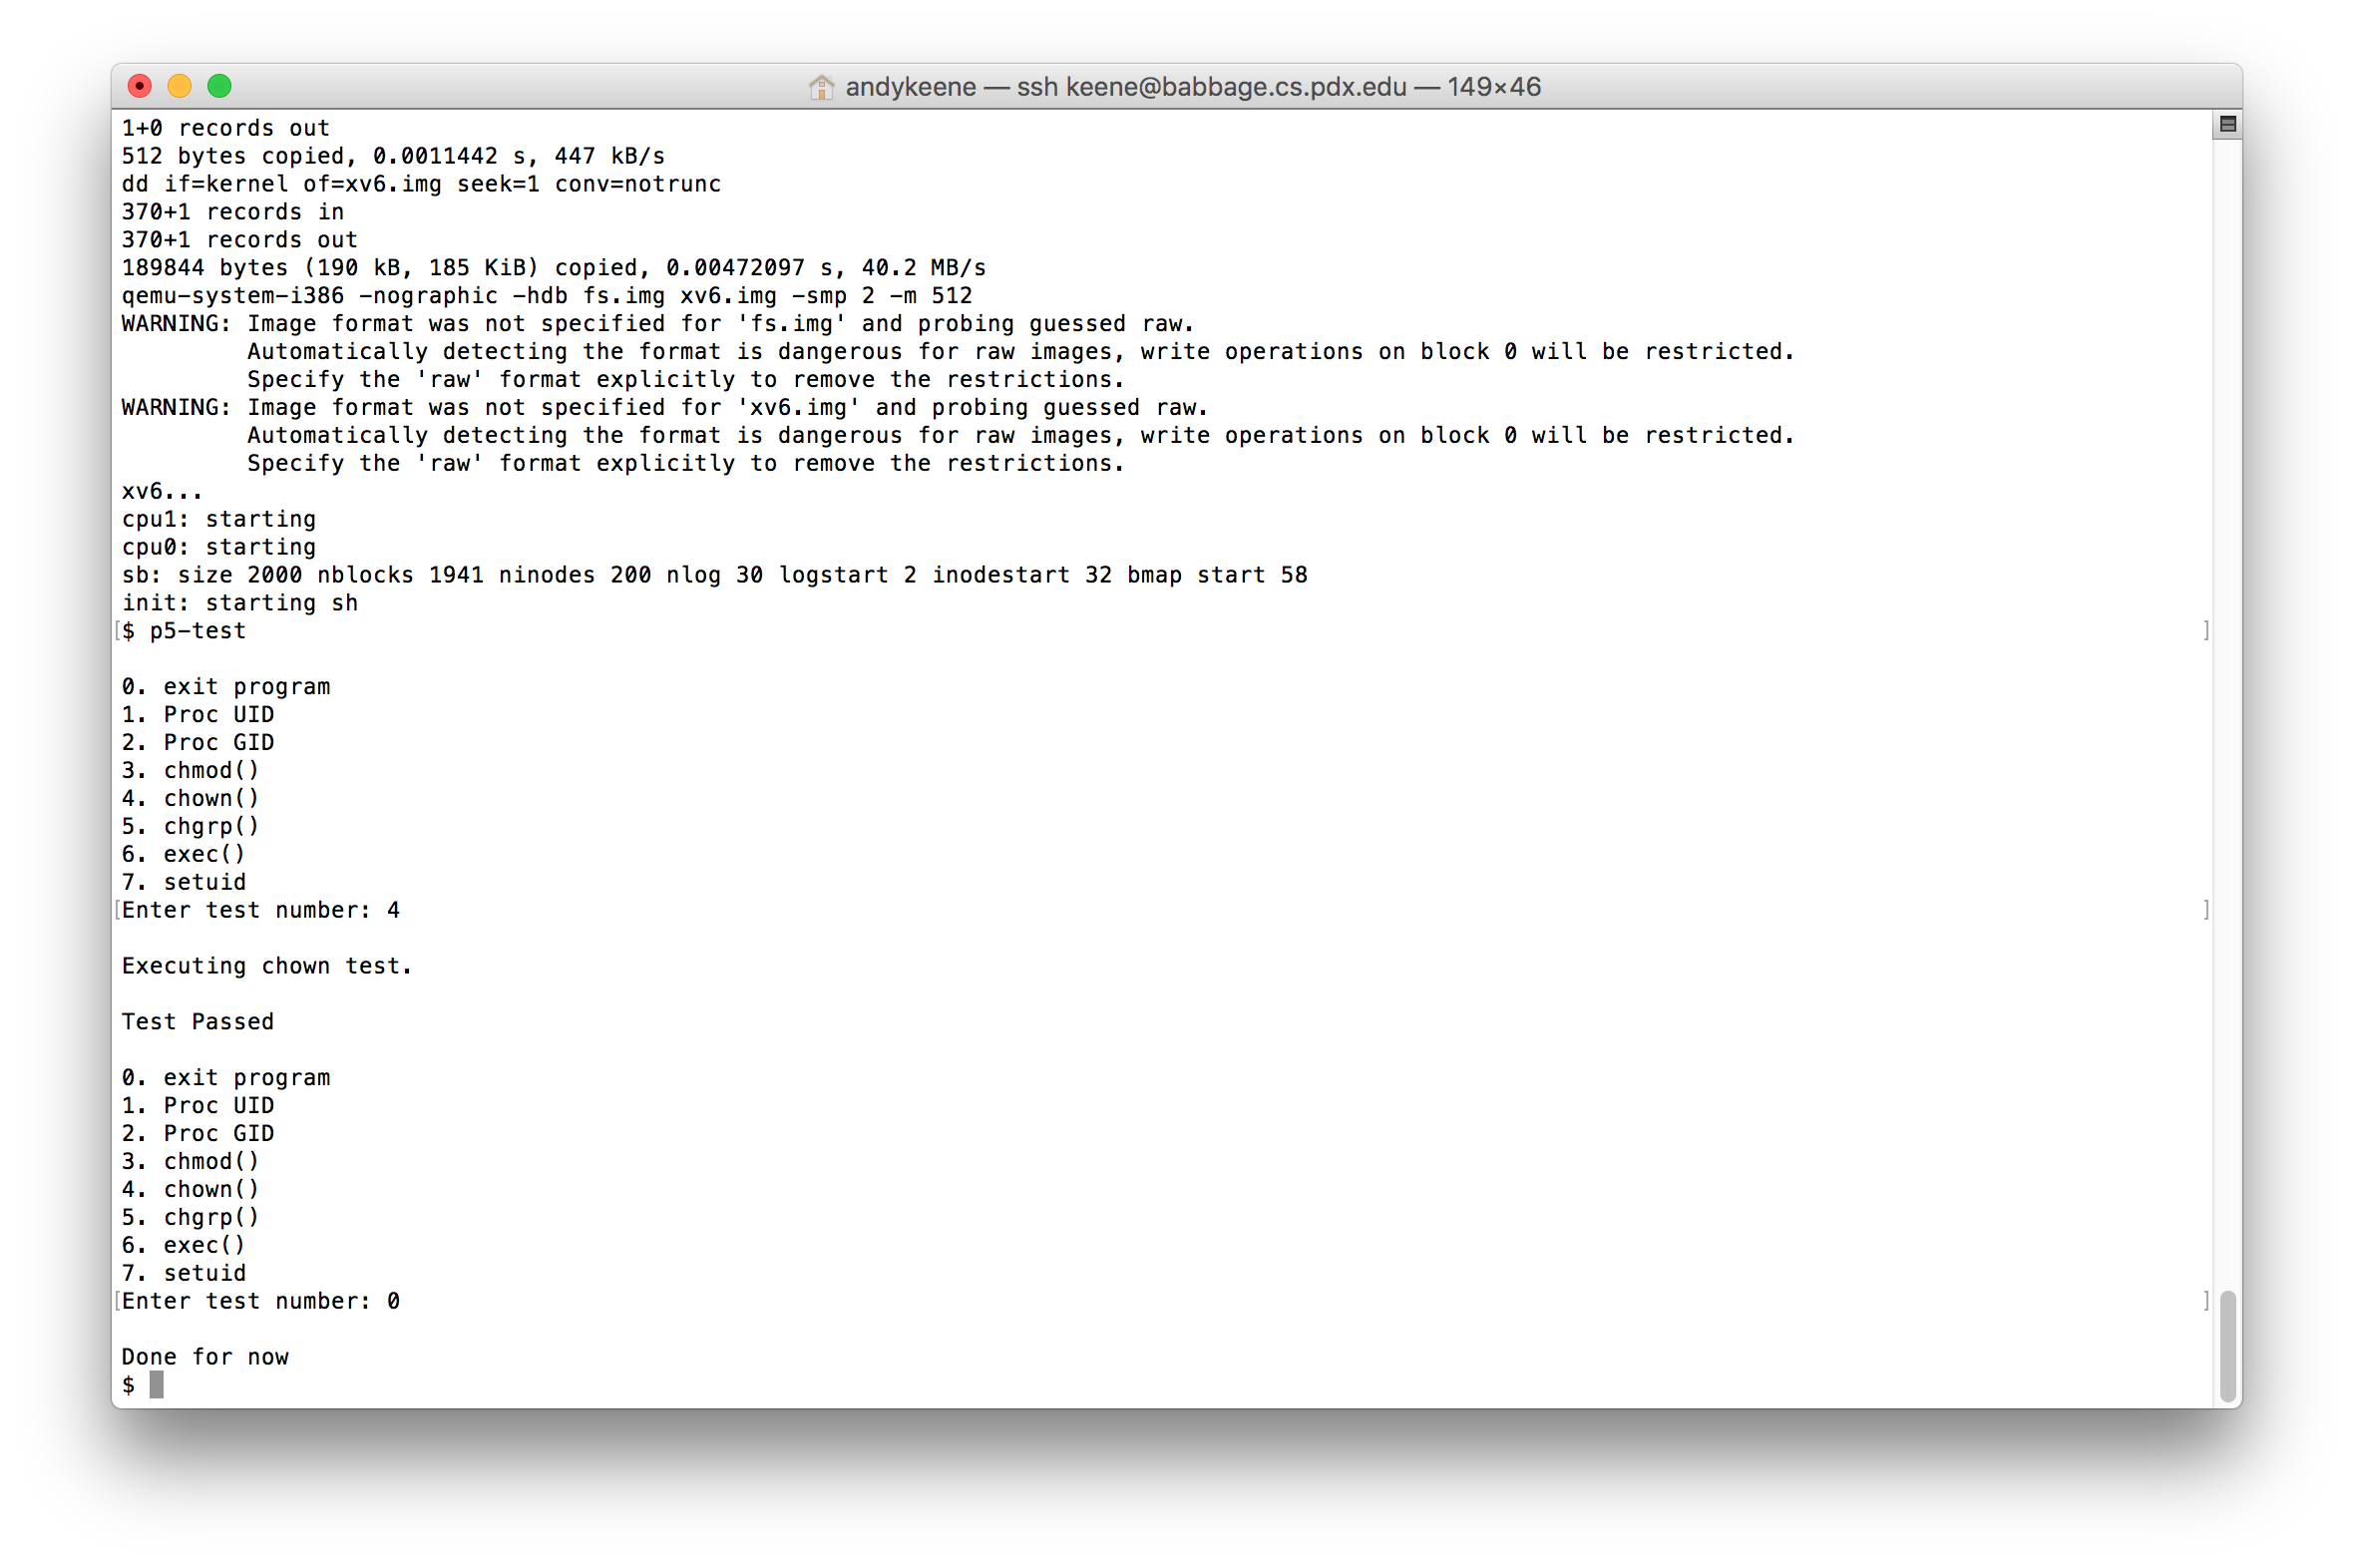
\includegraphics[width=0.8\linewidth]{dochowntest.png}
\caption{p5-test option 4: doChowntest()}
\label{fig:datetest}
\end{figure}

\pagebreak
Here we see that upon boot of xv6 that the program {\tt p5-test} was immediately run, and that by pressing 4 we invoked the specific test for {\tt doChownTest()}. Next we see that the test ran without
errors and that control was returned to the main menu as expected. Thus, since our expectations for this sub-test were met, this sub-test \textbf{PASSES}.
		
		
		\subsection{chgrp()}
		This test will demonstrate the correct behavior of the {\tt chgrp()} system call. To do this, we will run {\tt p5-test} immediately after the make and boot of xv6 
	and press 5 to trigger the function {\tt doChgrpTest()} with an argument of {\tt testsetuid} (described previously in \emph{0.0 System Calls}). 
	
	 {\tt doChgrpTest()} will notify us that is is executing then get the meta information for the file testsetuid by calling {\tt stat}. Next it will save the original GID, gid1, of
	 testsetuid before calling {\tt chgrp()} with an owner argument of gid1+1. Since during the file system creation all files are given a GID of $DEFAULT\_GID$ 
	 (demonstrated in test mkfs) which we 
	 know by virtue of code to be defined as 0 we can conclude that gid1+1 will in fact be within the valid bounds for a GID and consequently, the system call should succeed.
	 {\tt doChgrpTest()} then checks the return code of {\tt chgrp()} where an error message will be printed if the return code corresponds to an error. The file meta information
	 for testtestuid will then be refreshed with another call to stat. Using the stat structure, {\tt doChgrpTest()} will then ensure that the refreshed GID of the file matches the original
	 GID +1, or gid1+1 (this addition to the test occurs on line 256). Before returning control to the main loop {\tt doChgrpTest()} will reset the original file GID and print a message of success.
	 
	 We expect that after making and booting xv6 that when {\tt p5-test} is run and option 4 is selected that we will see only a message that {\tt doChgrpTest()} is running and 
	 a message that the test passed - by virtue of the code described for this test, will will know {\tt chgrp()} correctly updated the GID.

\begin{figure}[h!]
\centering
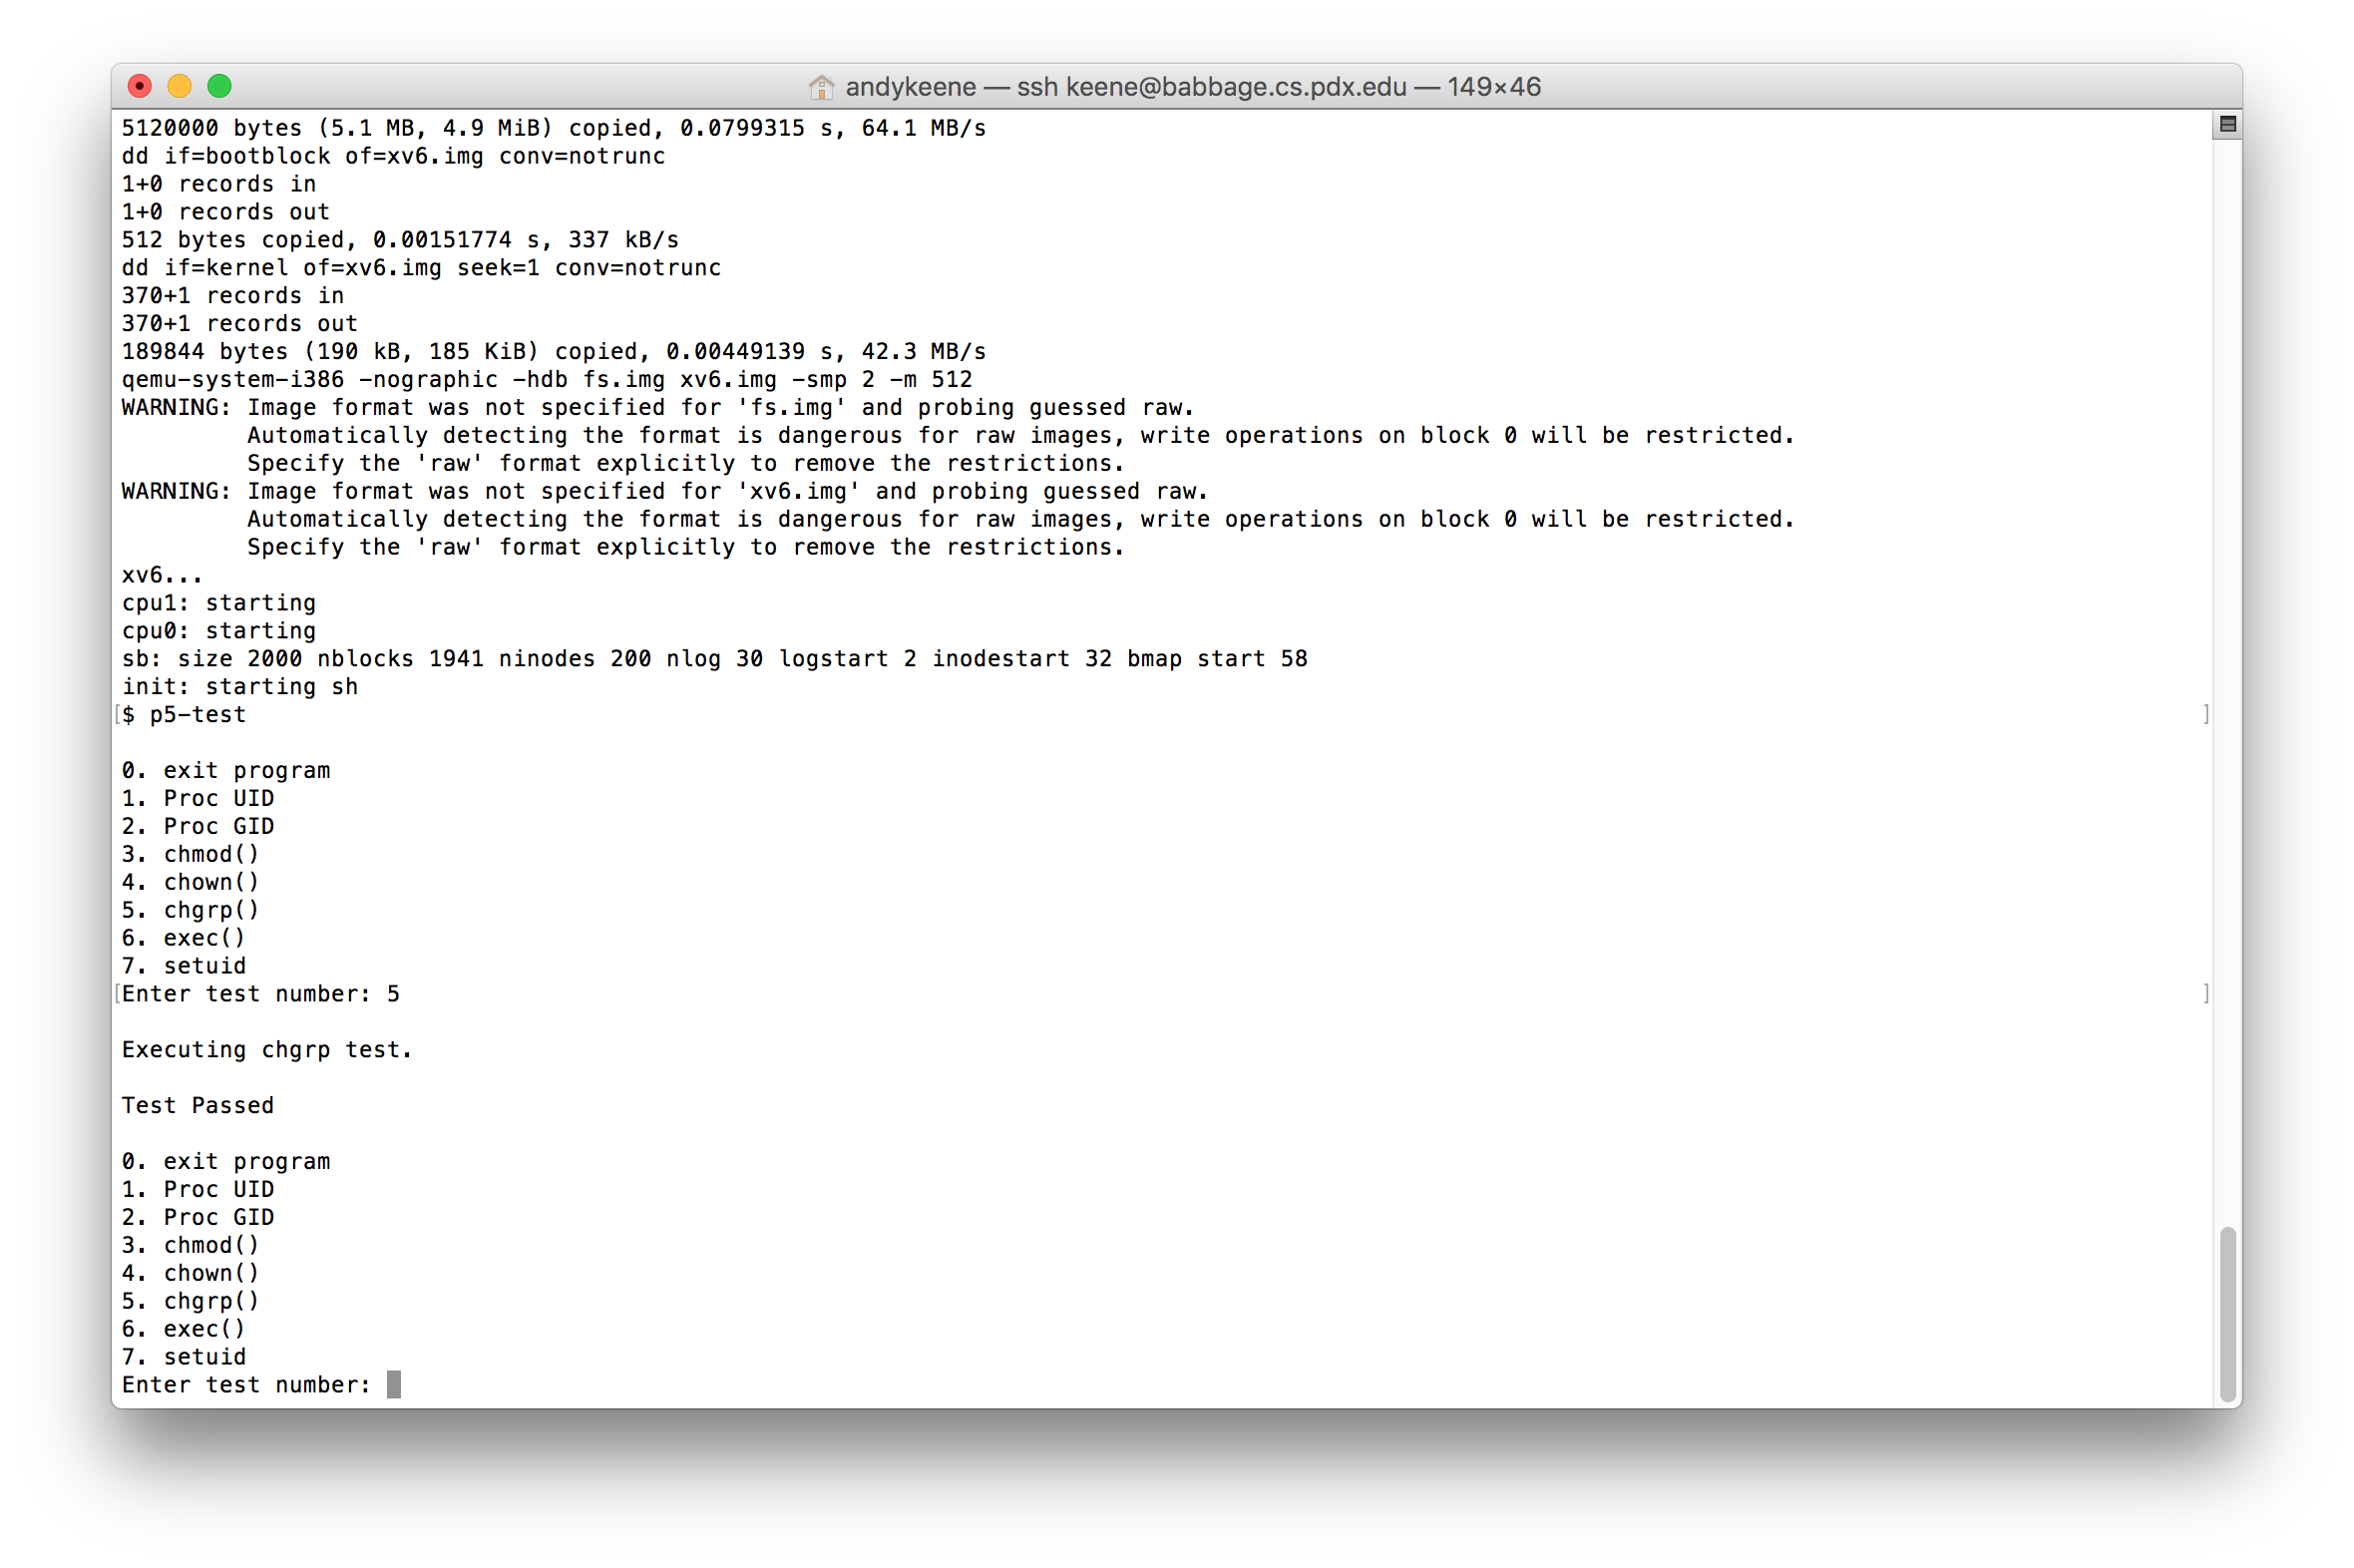
\includegraphics[width=0.8\linewidth]{dochgrptest.png}
\caption{p5-test option 5: doChowntest()}
\label{fig:datetest}
\end{figure}

\pagebreak
Here we see that upon boot of xv6 that the program {\tt p5-test} was immediately run, and that by pressing 5 we invoked the specific test for  {\tt doChgrpTest()}. Next we see that the test ran without
errors and that control was returned to the main menu as expected. Thus, since our expectations for this sub-test were met, this sub-test \textbf{PASSES}.	
		
		
		\subsection{exec()}
		This test will demonstrate the correct behavior of the {\tt exec()} system call. To do this, we will run {\tt p5-test} immediately after the make and boot of xv6 
	and press 6 to trigger the function {\tt doExecTest()} with an argument of {\tt testsetuid} (described previously in \emph{0.0 System Calls}). 	
		
	{\tt doExecTest()} will print that is running then will iteratively: set the UID and GID of the process; set the UID, GID, and mode of the file; then it will fork a child which will
	inherit its parents UID and attempt to execute, 
	via {\tt exec()}, the file testsetuid. If the fork or {\tt exec()} fail an error message will be printed. If the execution of testsetuid succeeds, the program will run and print 
	\emph{"***** In testsetuid: my uid is x"}. 
	
	Our expectations for {\tt doExecTest()} behavior for each of the following permission/UID/GID combos, done in-order, follow as:
	\begin{itemize}
	
		\item Only the file UID and process UID will be set to match with only executable permissions set for the owner - thus we expect the child process should be able to execute the testsetuid program.
		\item Only file GID and process GID will be set to match with only executable permissions set for the group - thus we expect the child process should be able to execute the testsetuid program.
		\item Neither the UID or GID of the file and process will be set to match, but executable permissions will be set for other - thus we expect the child process should be able to execute 
		the testsetuid program.
		\item Both the UID and GID for the field and process will be set to match but no executable permissions will be set - thus we expect the child process should \emph{not} be able to execute the testsetuid program.
	\end{itemize}
		Further, expectations for the successful execution of testsetuid will be printed by the child process to the screen prior to attempting {\tt exec()}.
\begin{figure}[h!]
\centering
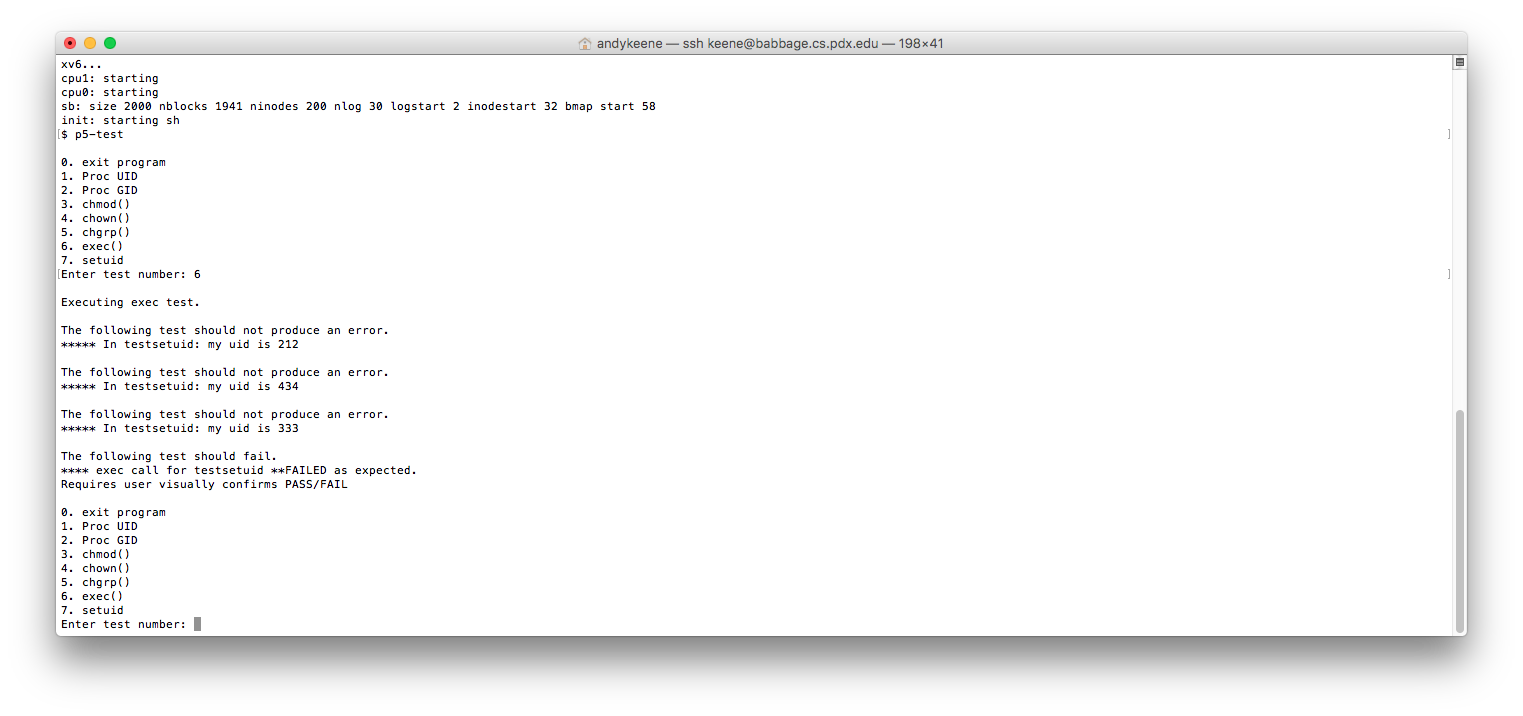
\includegraphics[width=0.8\linewidth]{doexectest.png}
\caption{p5-test option 6: doExectest()}
\label{fig:datetest}
\end{figure}

\pagebreak 

Here we see that upon a make and boot of xv6 that we ran option 6 of {\tt p5-test} and that {\tt doExecTest()} successfully completed. Further, we see that from
testsetuids execution and printing that the outlined expectations above (and reiterated within the test) are all met - the first three combinations of UID, GID, and permissions 
for {\tt exec()} succeed while the last fails. 
Thus, since each of our expectations for this test were met, this sub-test \textbf{PASSES}.
		
		
		\subsection{setuid flag}
		This test will demonstrate the correct behavior of the {\tt exec()} system call with the {\tt setuid} mode flag set. To do this, we will run {\tt p5-test} immediately after the make and boot of xv6 
	and press 7 to trigger the function {\tt doSetuidTest()} with an argument of {\tt testsetuid} (described previously in \emph{0.0 System Calls}).
		
		{\tt doSetuidTest} will follow the same setup procedure as test \emph{0.0.6 exec()} but in additional will now print the UID and GID for both the process and the file, 
		and print the files permissions (as base-10). Given the explicit list of permissions to be set as 1544, 1454, 1445, and 1666 and that
		the execution of {\tt testsetuid} is to print its UID, our modified expectations are as follows:
		
	\begin{itemize}
		\item Only the file UID and process UID will be set to match with only executable permissions set for the owner - thus we expect the child process should be able to execute the testsetuid program and since the setuid flag is set
			that testsetuid should print a UID that matches the file.
		\item Only file GID and process GID will be set to match with only executable permissions set for the group - thus we expect the child process should be able to execute the testsetuid program and since the setuid flag is set
			that testsetuid should print a UID that matches the file.
		\item Neither the UID or GID of the file and process will be set to match, but executable permissions will be set for other - thus we expect the child process should be able to execute 
		the testsetuid program and since the setuid flag is set
			that testsetuid should print a UID that matches the file.

		\item Both the UID and GID for the field and process will be set to match but no executable permissions will be set - thus we expect the child process should \emph{not} be able to execute the testsetuid program and no UID 
		should be printed.
	\end{itemize}

\begin{figure}[h!]
\centering
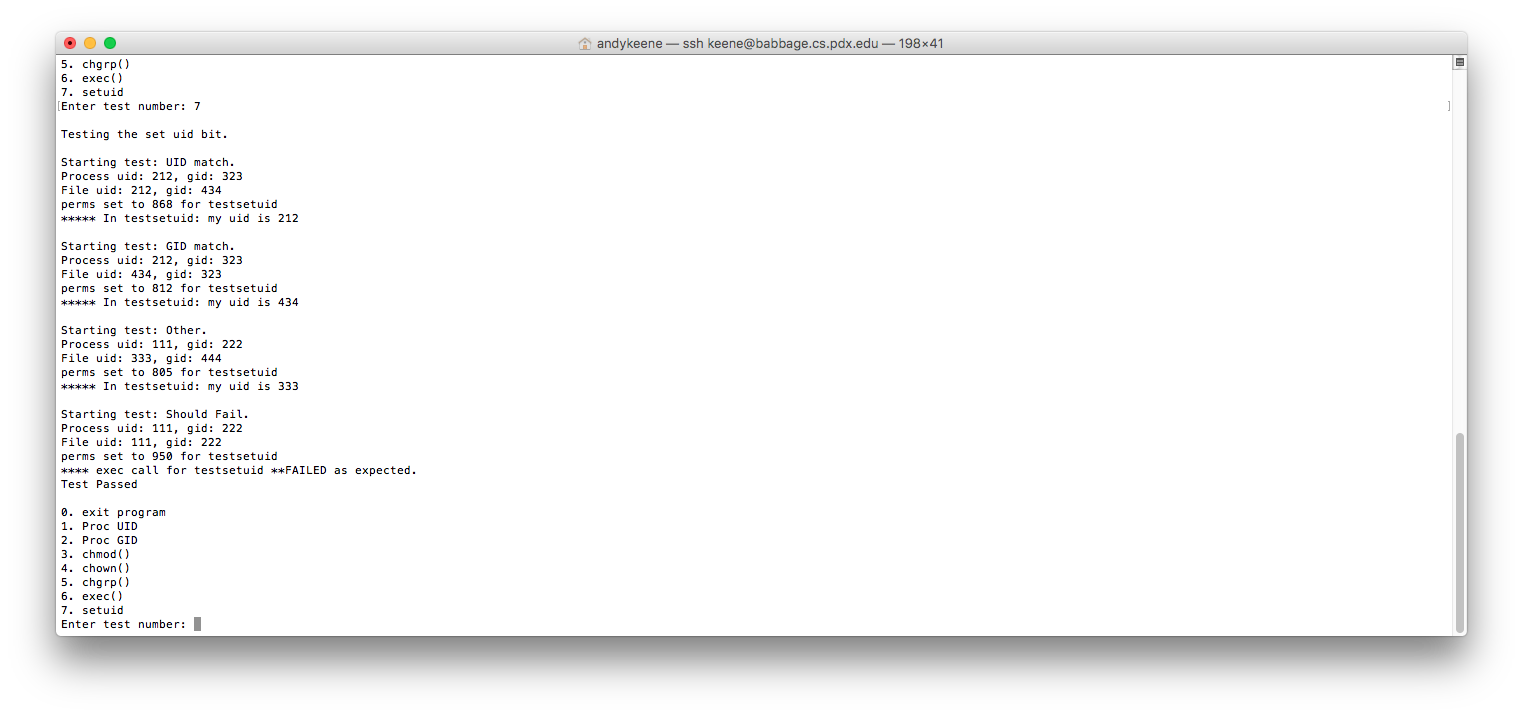
\includegraphics[width=0.8\linewidth]{dosetuidtest.png}
\caption{p5-test option 7: doSetuidTest()}
\label{fig:datetest}
\end{figure}	

\pagebreak

Here we see that: we ran {\tt p5-test} with option 7;  that the first three UID/GID/permission combinations where the process had executable permissions for the file testsetuid and the setuid flag was set, the program executed correctly 
and printed a UID that matched the file; 
that on the fourth execution (where no executable permissions were given) failed as expected; and that the test suite deemed {\tt doSetuidTest()} as passing. 
Thus since all of our expectations for each stage of the test were met we can conclude that this sub-test \textbf{PASSES}.

Since all sub-tests passed for the test \emph{System Calls}, we can conclude that the test \emph{System Calls} \textbf{PASSES}.

		\subsection*{Persistence}
		This test will demonstrate that any changes made to the file system persist after the xv6 kernel is shut down. To do this we will make and boot xv6, then display the filesystem contents
		with {\tt ls} which we expect to show the default files with the default UID of 0, GID of 0, and mode of 0755 (or -rwxr-xr-x). Next we will modify the UID, GID and mode of the default file
		README with values of 111, 222, and 0000 respectively. Next we will execute {\tt ls} again to show the expected effect of these changes on the current directory. We will then shut down
		xv6 with {\tt halt} and restart with {\tt make qemu-nox}; since the file system already exists, it will not trigger the {\tt mkfs} target in the Makefile and instead simply boot the previously
		 compiled version of xv6. Upon boot, since the file system was not rebuilt, we expect {\tt ls} to reflect that our previous changes persist for the README file.

\begin{figure}[h!]
\centering
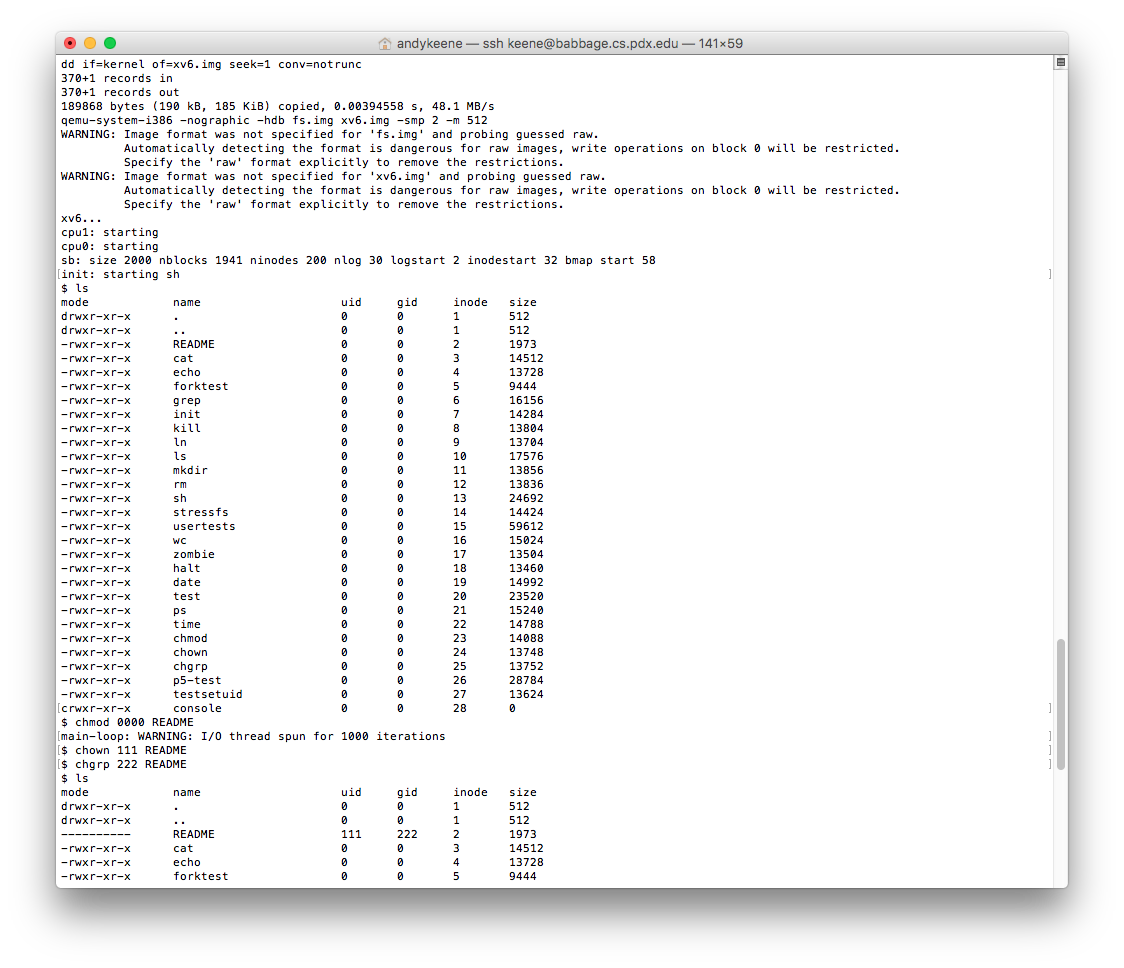
\includegraphics[width=0.8\linewidth]{persistence1.png}
\caption{First boot of xv6 with file contents}
\label{fig:datetest}
\end{figure}	

\pagebreak



\begin{figure}[h!]
\centering
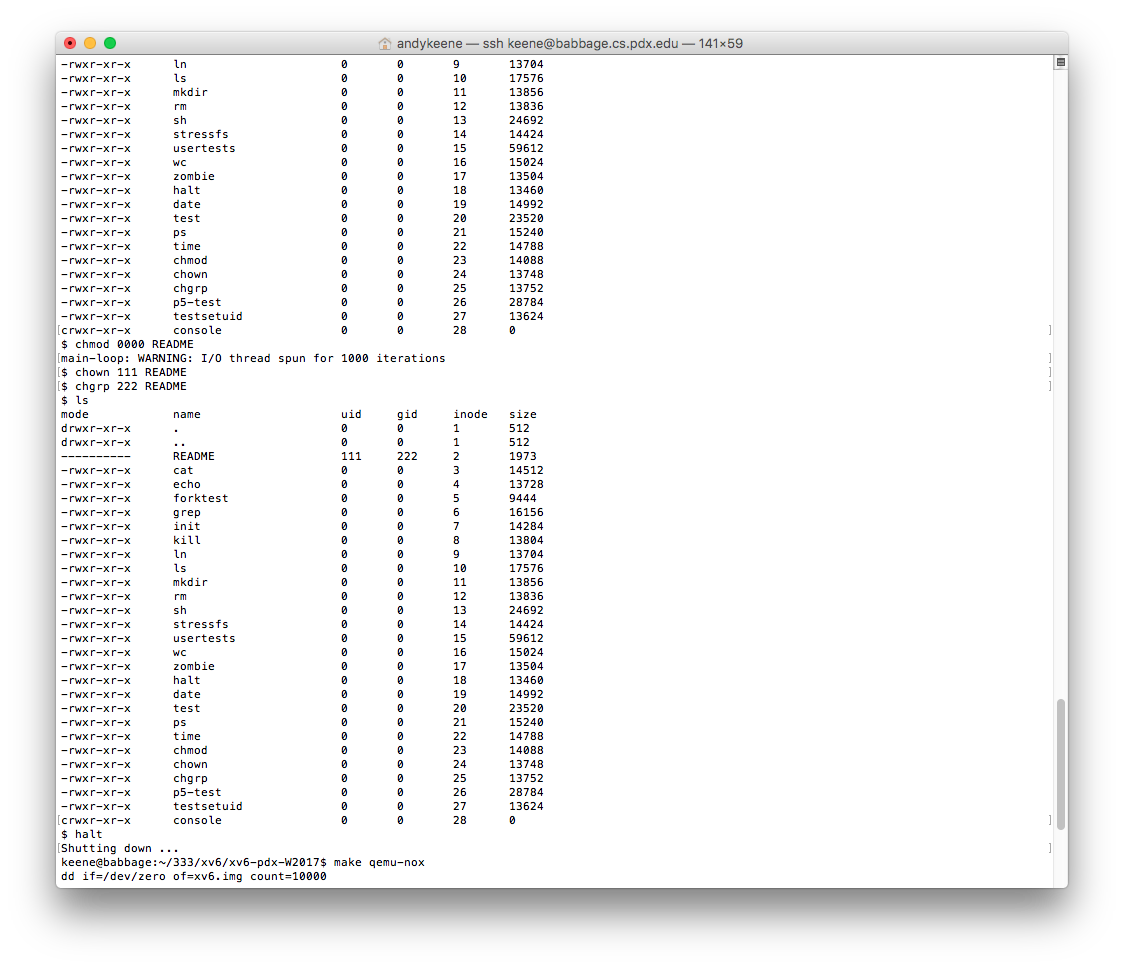
\includegraphics[width=0.8\linewidth]{persistence2.png}
\caption{Effect of changing REAME UID, GID and mode}
\label{fig:datetest}
\end{figure}	



\begin{figure}[h!]
\centering
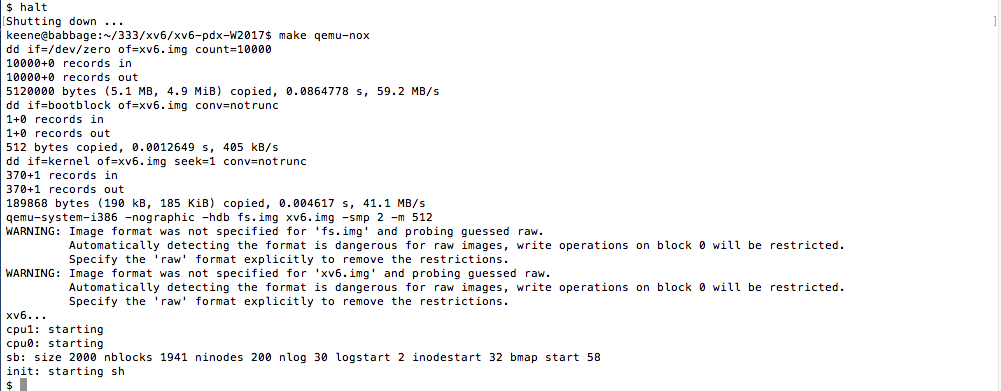
\includegraphics[width=0.8\linewidth]{persistence3.png}
\caption{Persistence after rebooting xv6}
\label{fig:datetest}
\end{figure}	

\pagebreak

Here we see in the three figures above that all files existed with the default permissions on the first boot of xv6; that {\tt ls} shows the file meta information for README change as expected; and that
after shutting down with {\tt halt} and restarting the system with {\tt make qemu-nox} that the changes we made persist. Thus, since our expectations for this sub-test were met, this 
sub-test \textbf{PASSES}.		 
		 
		
		
		\subsection*{User Commands}
		
		\subsection*{0.0.0 ls}
		This test will demonstrate that the user command {\tt ls} correctly prints the new associated information with file metadata - namely the inode number, GID, UID, and mode bits. To do 
		this we will make and boot xv6 then immediately list the contents of the current directory with {\tt ls}. Here we expect all default files to be listed in ascending inode numbering. We also
		expect that since all GID, UID, and mode values are set to the defaults of 0, 0, and 0755 respectively by the {\tt mkfs} program that each file will be listed with these values. It should be 
		noted that the mode 0755 corresponds to listing of permissions as {\tt -rwxr-xr-x}; however, the leading {\tt -} may differ since this is the indicator of whether the file is a directory (i.e. {\tt d}),
		a device like the console (i.e. {\tt c}), or simply a file (i.e. {\tt -}). We also expect, by virtue of the initial files not changing, that we will only see one directory, which is the root, under the
		names {\tt .} and {\tt ..} - these indicate the current and parent directory. The only device, {\tt c} that we expect to see is the console program responsible for handling interrupts.
		
		We will then use {\tt ls} to list the same meta information for a single file within the directory, README - here we expect that \emph{only} the meta information for README 
		will be listed with matching values of the initial {\tt ls} output. 
		
\begin{figure}[h!]
\centering
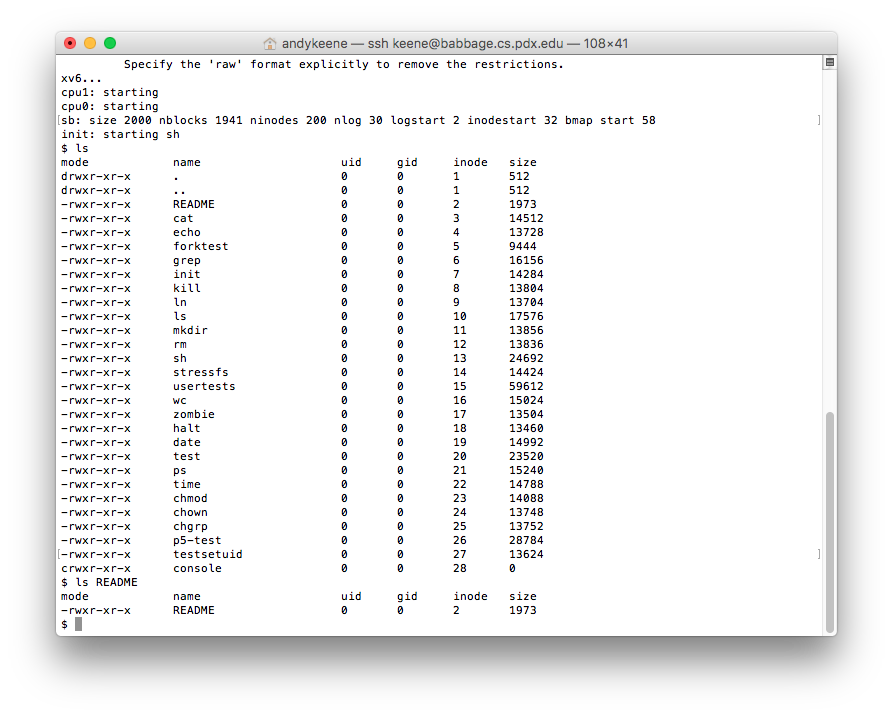
\includegraphics[width=0.8\linewidth]{ls.png}
\caption{ls}
\label{fig:datetest}
\end{figure}	 

\pagebreak

In the figure, \emph{ls}, above we see: that all files have the default permissions {\tt -rwxr-xr-x} with the exception of {\tt .} and {\tt ..} which contain a directory denotation and the console
file which contains a {\tt c} denotation; we also see that all inodes are listed in ascending order; that all files have the default UID and GID of 0; and that individual listing by {\tt ls} of README 
matches the initial output values and formatting. Thus, since all of our expectations were met we can conclude that this sub-test \textbf{PASSES}.

		%We will then create a new directory TEST-DIR with {\tt mkdir TEST-DIR}. We expect this directories mode to be listed 
		
		 		
		\subsection*{0.0.1 Valid Parameters for chmod, chown and chrp}
		This test will demonstrate that the user commands {\tt chmod}, {\tt chown}, and {\tt chgrp} change the mode, UID, and GID, respectively, of a file when passed in valid parameters (other than the defaults).
		To do this we will first boot xv6 and execute {\tt ls} to show the current file directory - note {\tt ls} was demonstrated as correct previously in the test \emph{ls}. Here we expect the files listed include the file \emph{cat} which is to 
		be used for our testing, and that all files will have the default
		mode 0755, the default GID of 0, and the default UID of 0 (by virtue of definitions in param.h). We will then:
		\begin{itemize}
			\item Invoke the command {\tt chmod 0777 cat} then execute {\tt ls} whose output we now expect to display the permissions {\tt -rwxrwxrwx} for cat.
			\item Invoke the command {\tt chown 19 cat} then execute {\tt ls} whose output we now expect to differ from the last only in the display of the UID {\tt 19} for cat.
			\item Invoke the command {\tt chgrp 88 cat} then execute {\tt ls} whose output we now expect to differ from the last only in the display of the GID {\tt 88} for cat.
		\end{itemize}


\begin{figure}[h!]
\centering
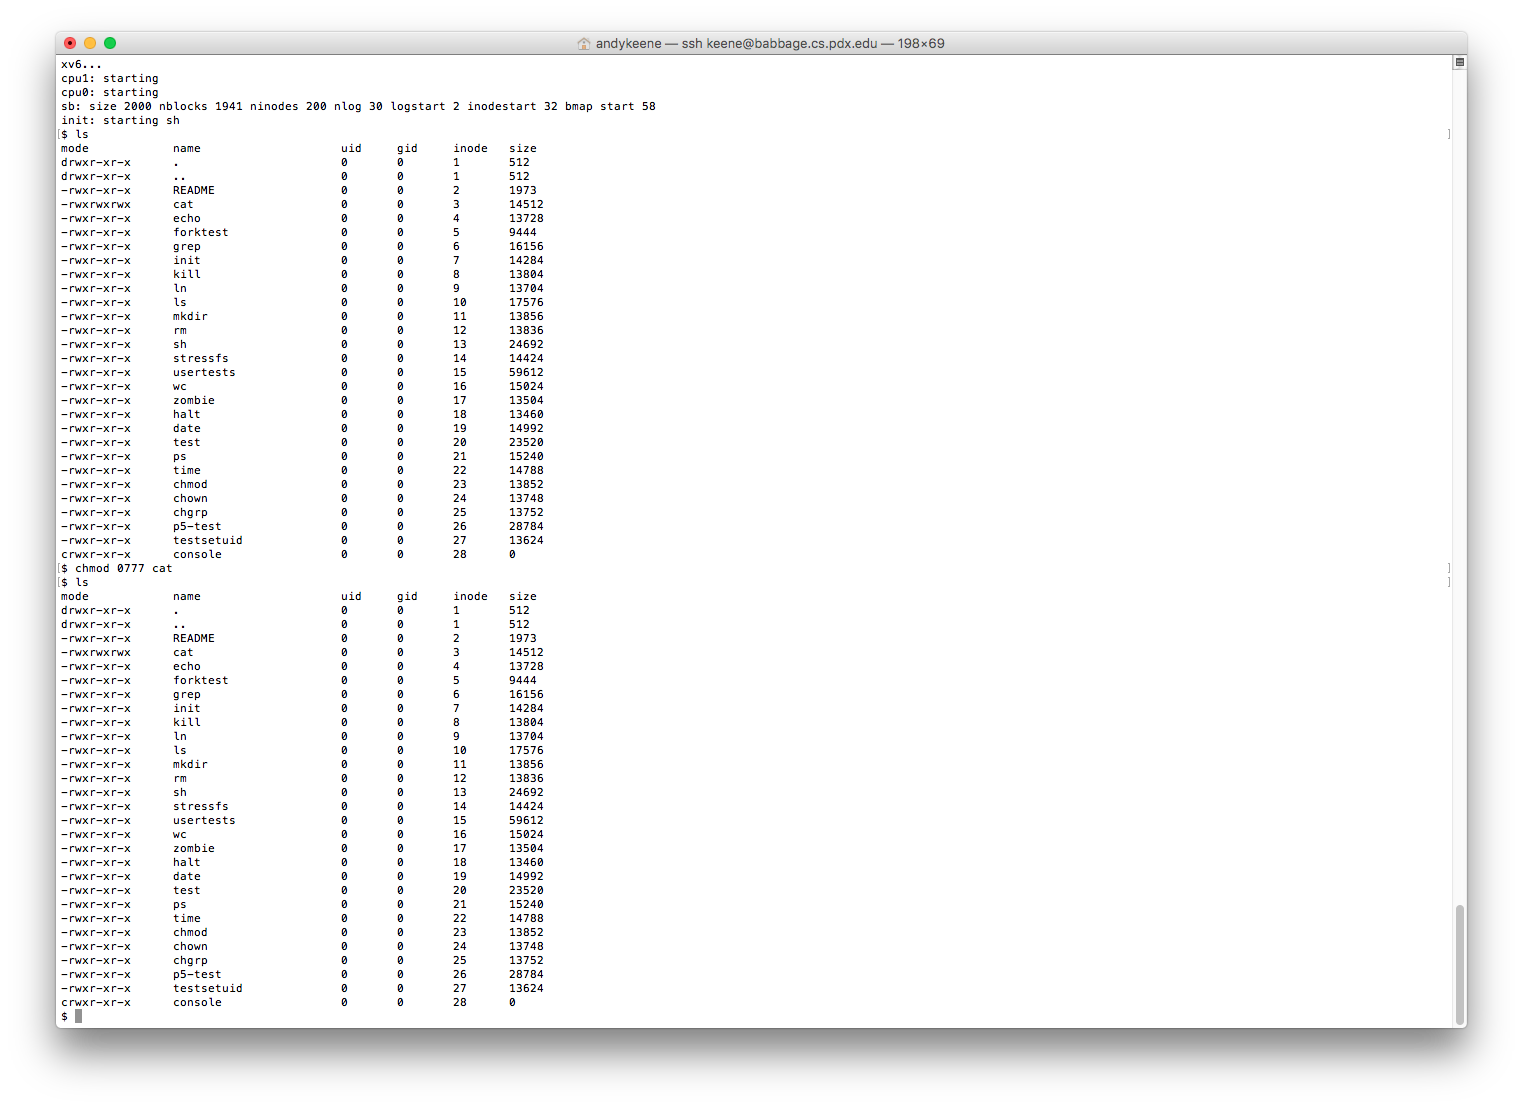
\includegraphics[width=0.8\linewidth]{validchmod.png}
\caption{chmod 0755 cat}
\label{fig:datetest}
\end{figure}

\pagebreak

\begin{figure}[h!]
\centering
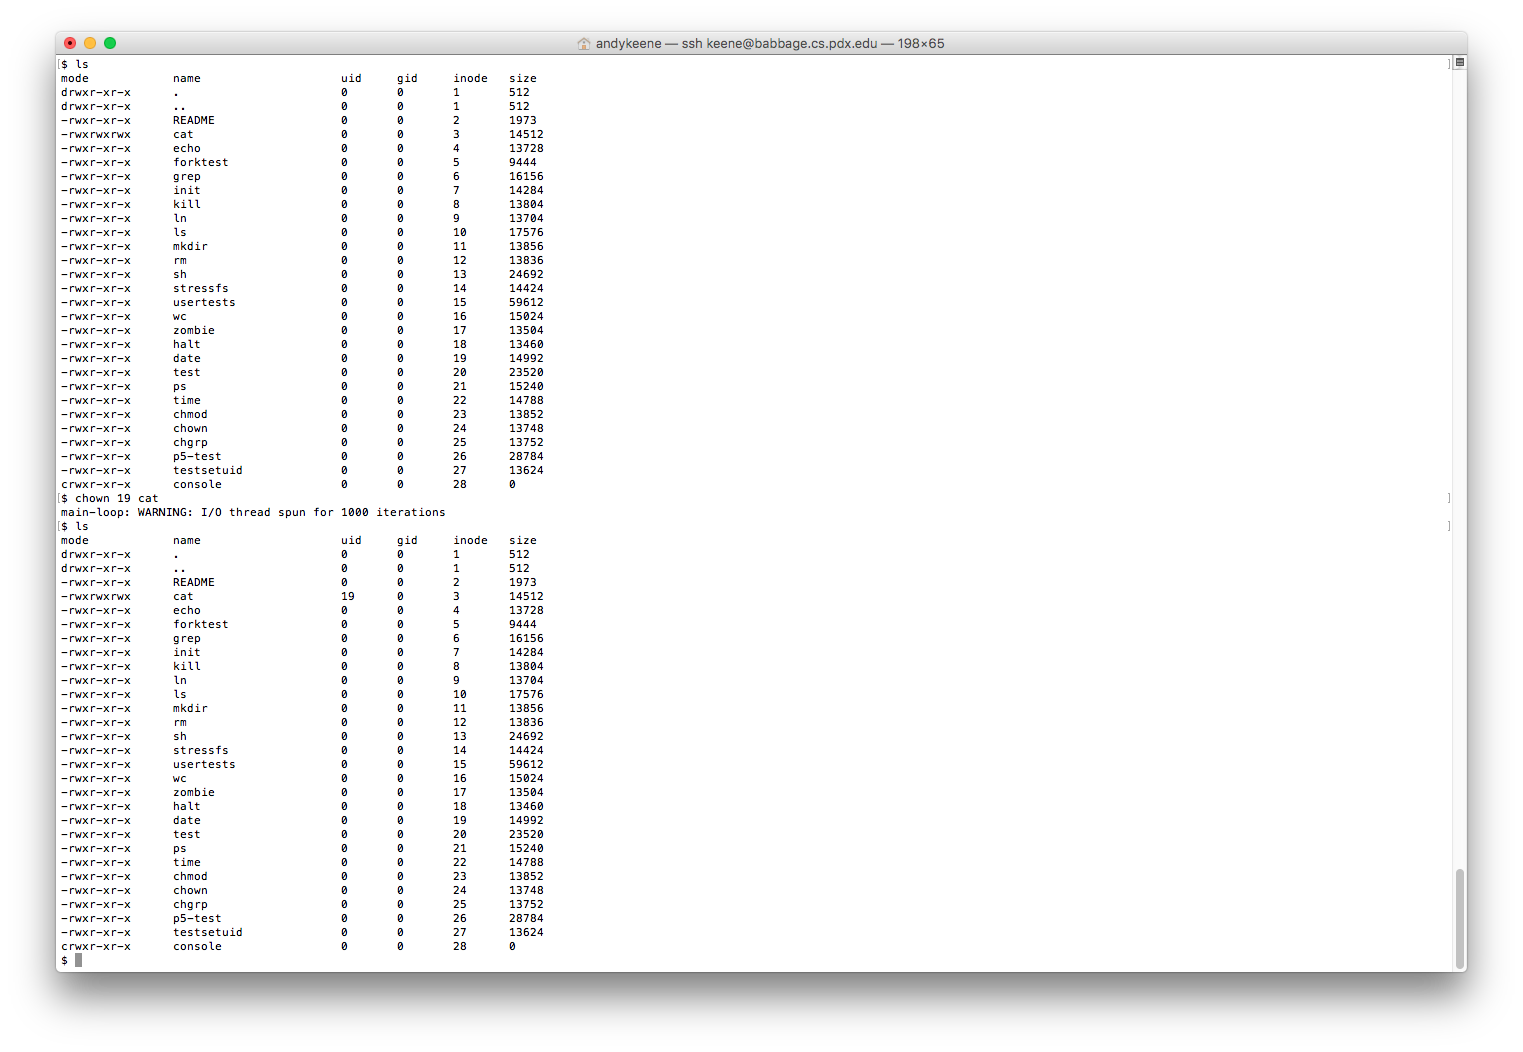
\includegraphics[width=0.8\linewidth]{validchown.png}
\caption{chown 19 cat}
\label{fig:datetest}
\end{figure}

\pagebreak

\begin{figure}[h!]
\centering
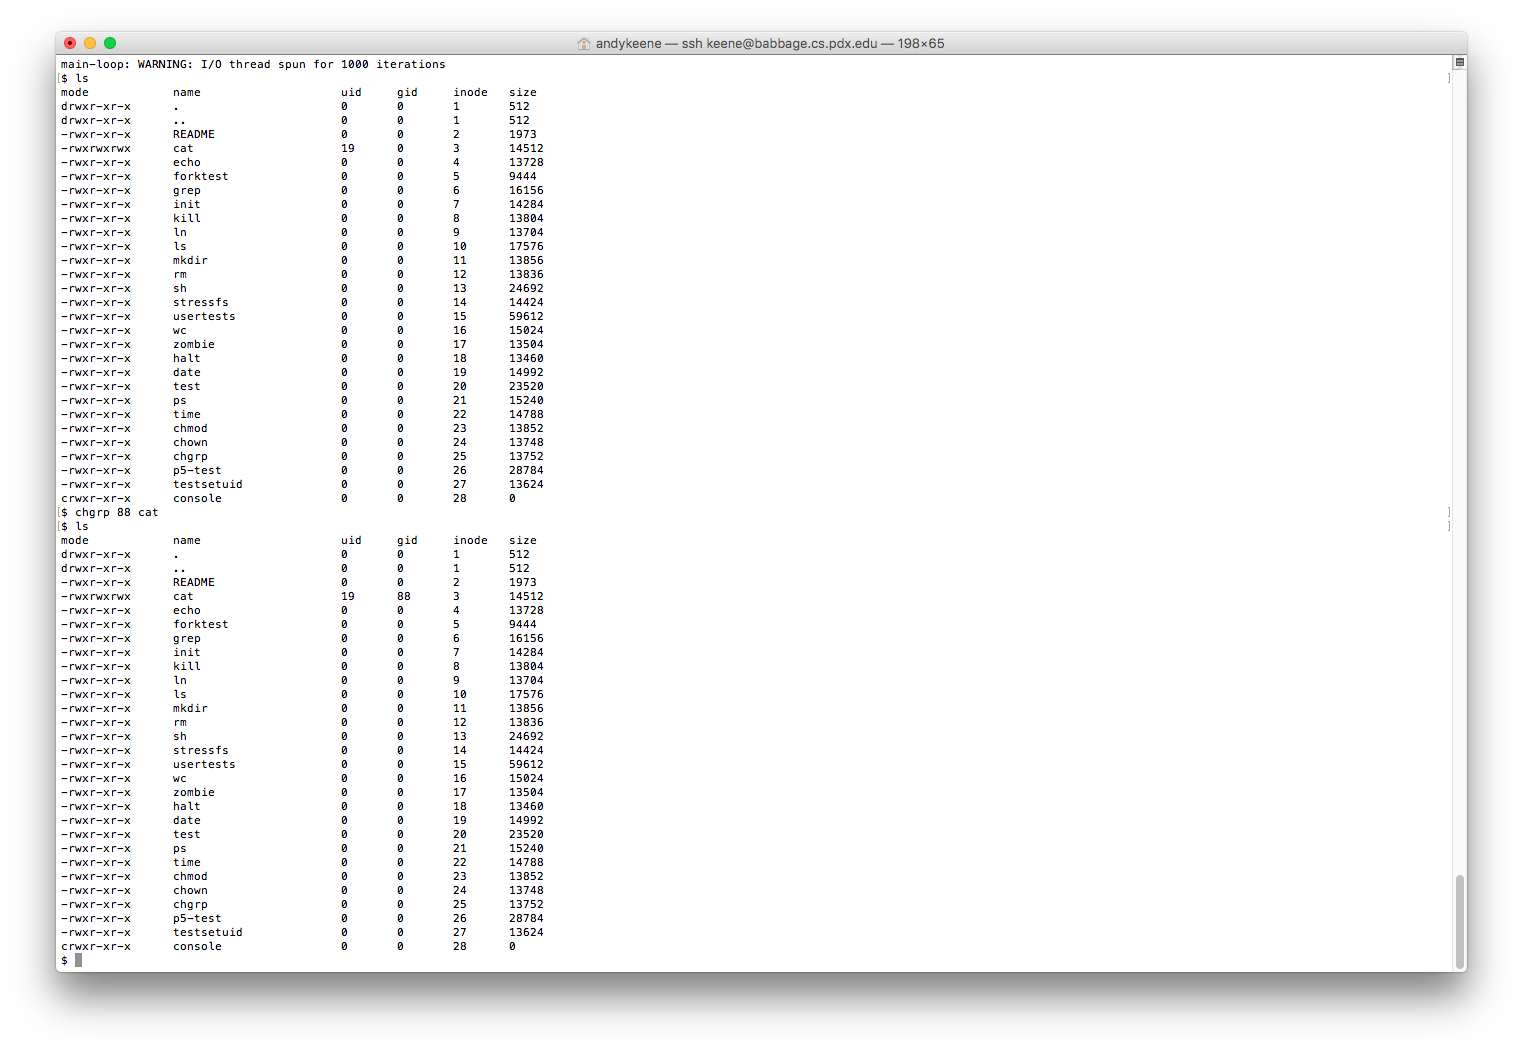
\includegraphics[width=0.8\linewidth]{validchgrp.png}
\caption{chgrp 88 cat}
\label{fig:datetest}
\end{figure}

\pagebreak


We see that immediately after boot that the file cat does in fact exist in the current directory with the default mode of 0755, the default UID of 0, and the default GID of 0. We also see that after execution of {\tt chmod 0777 cat}
that the file then has the correct corresponding permissions  {\tt -rwxrwxrwx}; that after the execution of {\tt chown 19 cat} the file has the correct UID of 19; and that after the execution of {\tt chgrp 88 cat} that the file has the correct
GID of 88. Thus all of our expectations were met. Since all of our expectations were met, this sub-test \textbf{PASSES}.

	\subsection*{0.0.2 Invalid filename parameter for chmod, chown and chrp}

	This test will demonstrate that the user commands {\tt chmod}, {\tt chown}, and {\tt chgrp} do not modify any file when given an invalid filename.
		To do this we will first boot xv6 and execute {\tt ls} to show the current file directory - note {\tt ls} was demonstrated as correct previously in the test \emph{ls}. We will then choose a filename that does not exist in the
		directory, such as TEST-INVALID, and execute the user commands {\tt chmod}, {\tt chown}, and {\tt chgrp} with the valid numeric parameters 0777, 19, and 88, but with the invalid filename TEST-INVALID. The behavior for
		these user commands with valid parameters was demonstrated correct in the previous test \emph{Valid Parameters for chmod, chown and chrp} which will demonstrate that any failure here is due strictly to an invalid filename.
		Since, by the construction of these user commands an error message will be printed upon an unsuccessful return code of the system call, we expect after the execution of each command  {\tt chmod}, {\tt chown}, and {\tt chgrp} 
		to print an error message. We will then execute {\tt ls} again, and expect the output to be identical to the the first.
		
		
\begin{figure}[h!]
\centering
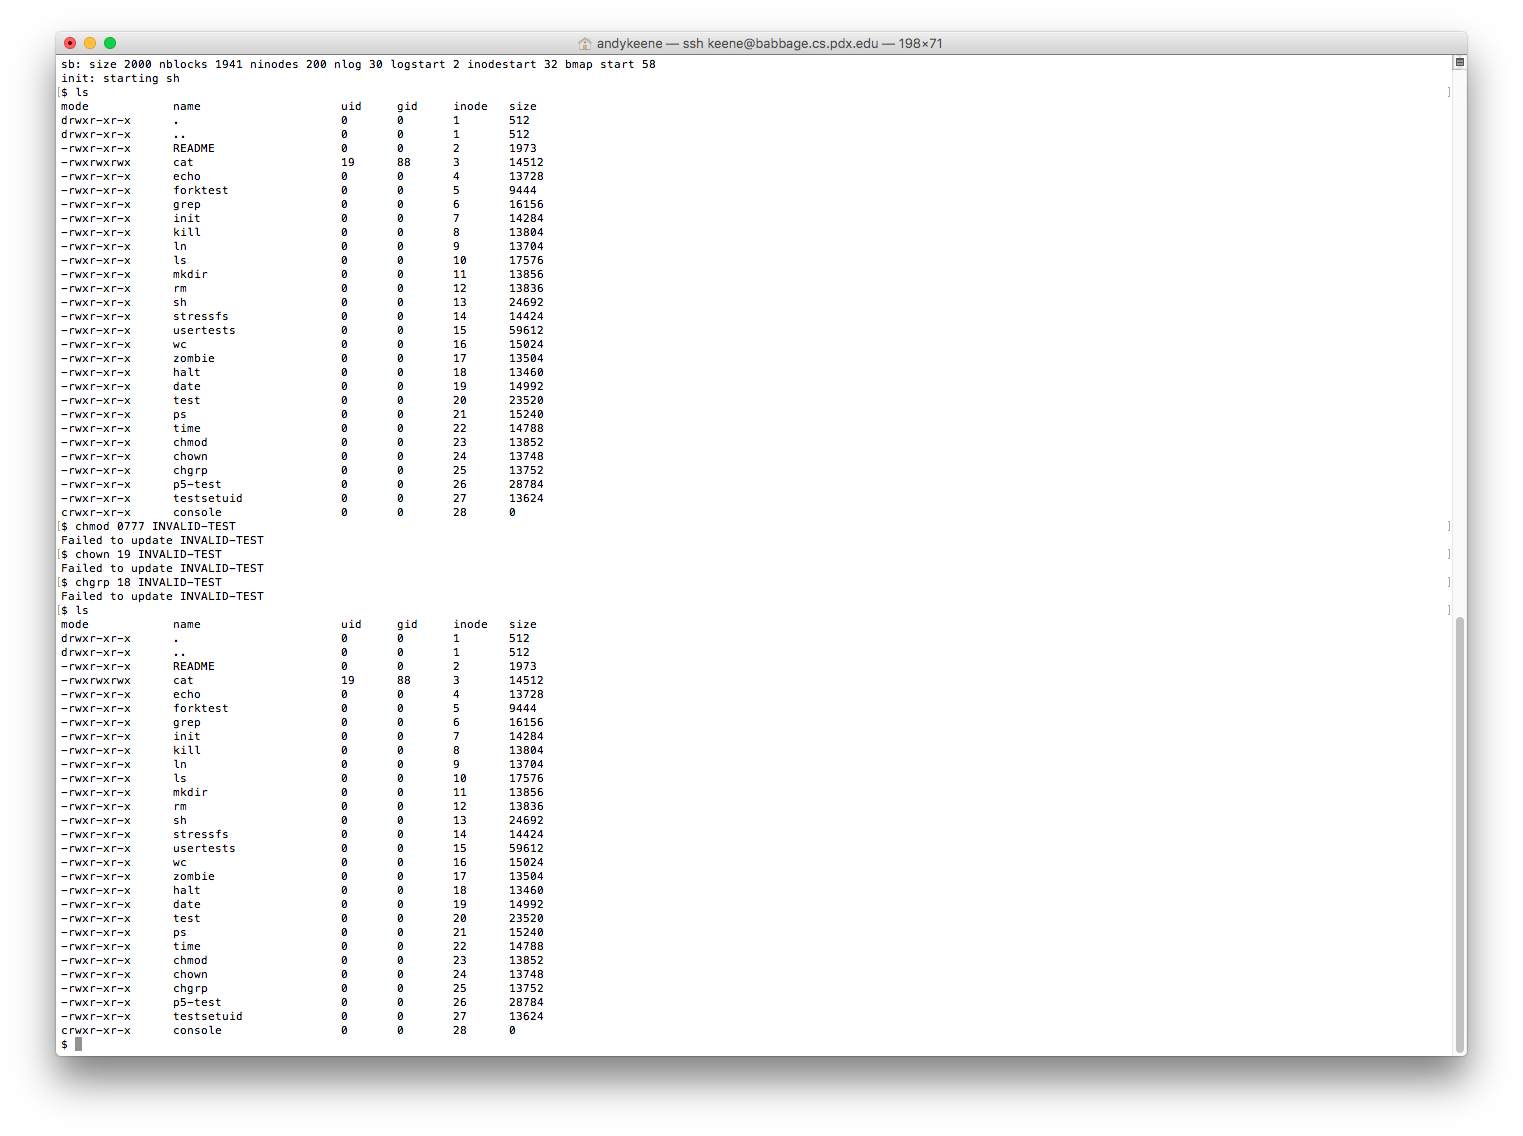
\includegraphics[width=0.8\linewidth]{invalidfilename.png}
\caption{Invalid Filename Parameter}
\label{fig:datetest}
\end{figure}

\pagebreak

Here we see that the output from {\tt ls} immediately after xv6 booted is identical to its output after the attempted user commands and that the file INVALID-TEST did not exist; further we see that each attempted user command with 
the invalid filename parameter printed the error message \emph{"Failed to update INVALID-TEST"}. Thus, since our expectations for this sub-test are met we can conclude that this sub-test \textbf{PASSES}. 


		\subsection*{0.0.3 Invalid numeric parameter for chmod, chown and chrp}
		This test will demonstrate that the user commands {\tt chmod}, {\tt chown}, and {\tt chgrp} do not modify any file when given an invalid numeric parameter.
		To do this we will first boot xv6 and execute {\tt ls} to show the current file directory - note {\tt ls} was demonstrated as correct previously in the test \emph{ls}. We will then choose a filename that exists in the
		directory, such as cat, and execute the user command {\tt chmod}, {\tt chown}, and {\tt chgrp} with the invalid numeric parameters 0877, -1, and 32768 respectively, but with the \emph{valid} filename cat. The behavior for
		these user commands with valid parameters was demonstrated correct in the previous test \emph{Valid Parameters for chmod, chown and chrp} which will demonstrate that any failure here is due strictly to an invalid numeric parameter.
		Since, by the construction of these user commands an error message will be printed upon an unsuccessful return code of the system call, we expect after the execution of each command  {\tt chmod}, {\tt chown}, and {\tt chgrp} 
		to print an error message; specifically we expect {\tt chown}, and {\tt chgrp} to print \emph{"Failed to update cat"} and {\tt chmod} to print \emph{"Invalid MODE"}. 
		
		We will then execute {\tt ls} again, and expect the output to be identical to the the first.
		
\begin{figure}[h!]
\centering
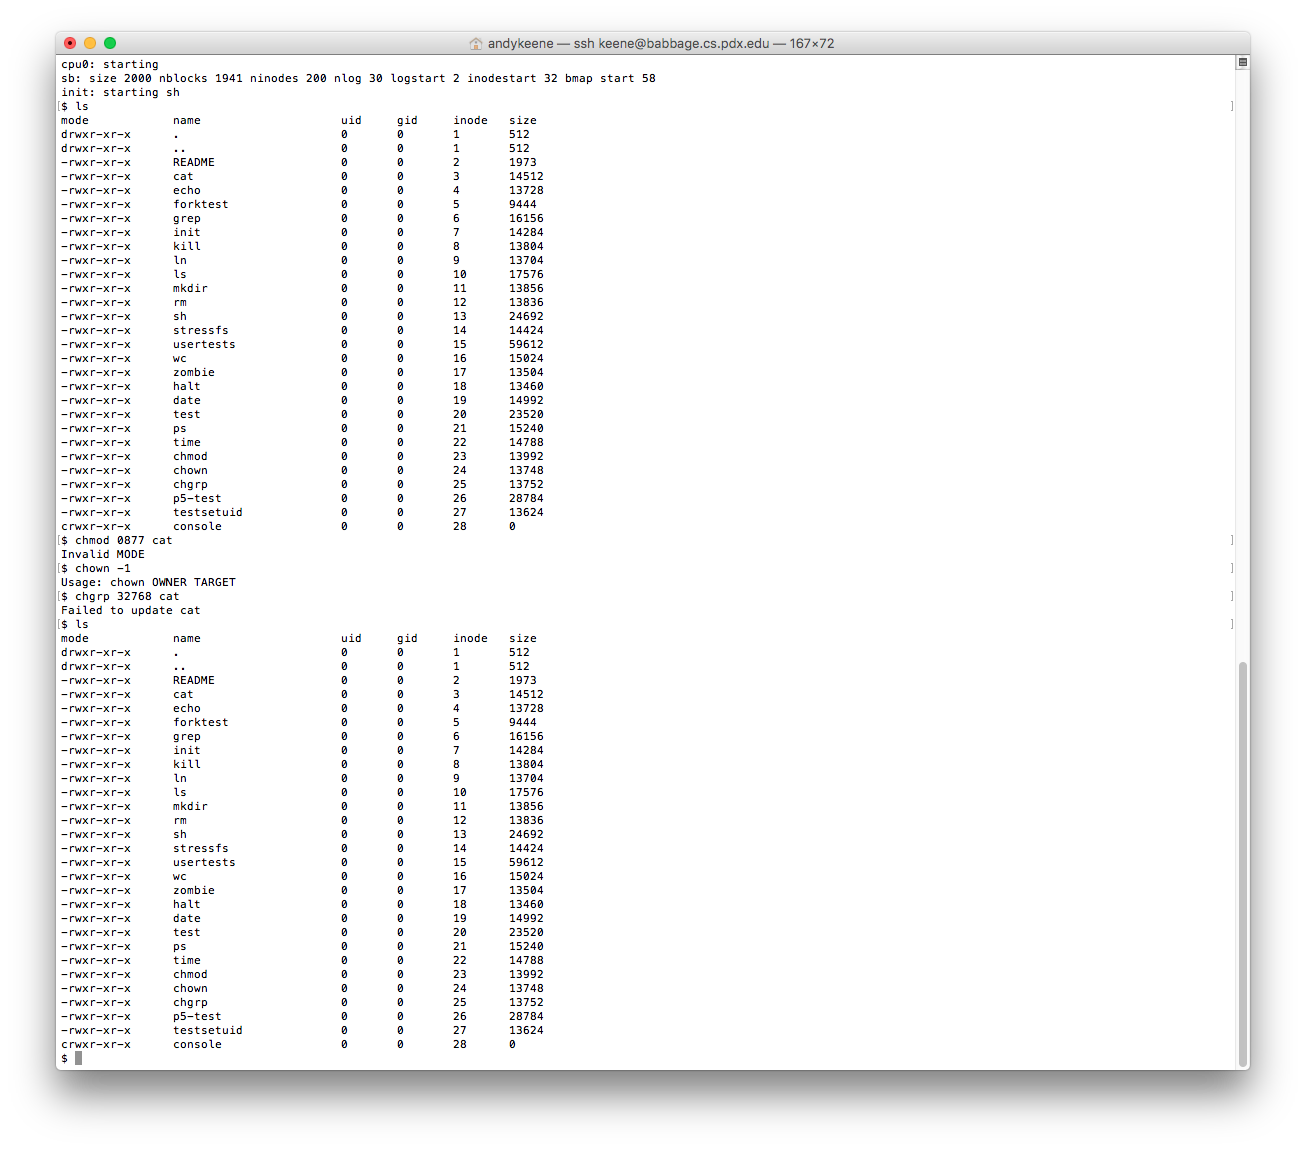
\includegraphics[width=0.8\linewidth]{invalidnumeric.png}
\caption{Invalid Numeric Parameter}
\label{fig:datetest}
\end{figure}


\pagebreak
In the figure above we see that immediately after xv6 is booted that {\tt ls} shows cat is in the current directory with default the permissions, GID, and UID. Next we see that as expected {\tt chmod}, {\tt chown}, and {\tt chgrp} 
respond to our invalid numeric parameters with the appropriate messages \emph{"Failed to update cat"} and \emph{"Invalid MODE"}; where further we see the 
second {\tt ls} output is identical to the first, showing that no attempts to change the files meta information were successful. Since all of our expectations for this sub-test were met we can conclude
that this sub-test \textbf{PASSES}.

This all sub-tests for \emph{User Commands} passed, we can conclude that this test \textbf{PASSES}
		
\end{document}




